\documentclass[11pt, oneside]{article}

\usepackage[english]{babel}
\usepackage{geometry}  
\usepackage{graphicx}      
\usepackage{tabularx}      
\usepackage{amssymb}
\usepackage{amsmath}
\usepackage{booktabs}
\usepackage{hyperref}
\usepackage{achemso}
\usepackage{csquotes}
\usepackage{cleveref}
\usepackage{siunitx}
\usepackage{geometry}
\geometry{left=4cm, right=4cm}

\usepackage[dvipsnames]{xcolor}
\definecolor{tumblue}{rgb}{0,0.396078431372549,0.741176470588235}

\usepackage{xspace}
\usepackage{caption}
\usepackage{subcaption}
\usepackage{authblk} 

\usepackage{sectsty} 
\usepackage[acronym]{glossaries}
\usepackage[sort&compress,numbers,super]{natbib}

\sectionfont{\color{tumblue}\selectfont\sffamily}
\subsectionfont{\color{tumblue}\selectfont\sffamily}
\subsubsectionfont{\color{tumblue}\selectfont\sffamily}
\paragraphfont{\selectfont\sffamily}
\subparagraphfont{\color{gray}\selectfont\sffamily}


\renewcommand*{\Authfont}{\sf}
\renewcommand*{\Affilfont}{\sf}


\definecolor{halfgray}{gray}{0.55}
\renewcommand\labelitemi{\color{halfgray}$\bullet$} 

 
\usepackage{kpfonts}
\usepackage{biolinum}

\clubpenalty = 10000 
\widowpenalty = 10000 
\displaywidowpenalty = 10000


\usepackage{lipsum}
\usepackage[labelfont=bf]{caption}

\newacronym{llm}{LLM}{large language model}
\newacronym{ml}{ML}{machine learning}
\newacronym{agi}{AGI}{artificial general intelligence}
\newacronym{api}{API}{application programming interface}
\newacronym{mcq}{MCQ}{multiple-choice question}
\newacronym{rest}{REST}{Representational State Transfer}
\newacronym{orm}{ORM}{object relational mapping}
\newacronym{dai}{DAI}{daily allowed intake}
\newacronym{ghs}{GHS}{Globally Harmonized System of Classification and Labelling of Chemicals}
\newacronym{who}{WHO}{World Health Organization}
\newacronym{nmr}{NMR}{Nuclear Magnetic Resonance}
\newacronym{helm}{HELM}{Holistic Evaluation of Language Models}
\newacronym{smiles}{SMILES}{Simplified Molecular Input Line-Entry System}
\newacronym{pca}{PCA}{Principal Component Analysis}
\newacronym{iupac}{IUPAC}{International Union of Pure and Applied Chemistry}
\newacronym{json}{JSON}{JavaScript Object Notation}
\usepackage{credits}
\usepackage{orcidlink}
\usepackage{showyourwork}


\title{\textsf{Are frontier models superhuman chemists?}}

%Conceptualization
%Data curation
%Formal analysis - Application of statistical, mathematical, computational, or other formal techniques to analyse or synthesize study data.
%Funding acquisition
%Investigation - Conducting a research and investigation process, specifically performing the experiments, or data/evidence collection.
%Methodology
%Project administration
%Resources
%Software
%Supervision
%Validation
%Visualization
%Writing -- original draft
%Writing -- review & editing


% Main contributors
\credit{Adrian~Mirza}{1,1,1,0,1,0,0,0,1,0,1,1,0,1}
\credit{Nawaf~Alampara}{1,1,1,0,1,0,0,0,1,0,1,0,0,1}
\credit{Sreekanth~Kunchapu}{1,1,0,0,1,0,0,0,0,0,1,0,0,1}
\credit{Martiño~Ríos-García}{1,1,1,0,1,0,0,0,1,0,1,0,0,1}


% Question contributors
\credit{Benedict~Emoekabu}{0,1,0,0,1,0,0,0,0,0,0,0,0,1}
\credit{Aswanth~Krishnan}{0,0,0,0,0,0,0,0,1,0,0,0,0,1}
\credit{Tanya~Gupta}{0,1,0,0,1,0,0,0,0,0,0,0,0,1}
\credit{Mara~Wilhelmi}{0,1,0,0,1,0,0,0,0,0,0,0,0,1}
\credit{Macjonathan~Okereke}{0,1,0,0,1,0,0,0,0,0,0,0,0,1}


% Question answerers
\credit{Mehrdad Asgari}{0,1,0,0,0,0,0,0,0,0,0,0,0,1}
\credit{Juliane Eberhardt}{0,1,0,0,0,0,0,0,0,0,0,0,0,1}
\credit{Amir~Mohammad~Elahi}{0,1,0,0,0,0,0,0,0,0,0,0,0,1}
\credit{Hani~M.~Elbeheiry~}{0,1,0,0,0,0,0,0,0,0,0,0,0,1}
\credit{María~Victoria~Gil}{0,1,0,0,1,0,0,0,0,0,0,0,0,1}
\credit{Christina Glaubitz}{0,1,0,0,0,0,0,0,0,0,0,0,0,1}
\credit{Maximilian Greiner}{0,1,0,0,0,0,0,0,0,0,0,0,0,1}
\credit{Caroline T. Holick}{0,1,0,0,0,0,0,0,0,0,0,0,0,1}
\credit{Tim Hoffmann}{0,1,0,0,0,0,0,0,0,0,0,0,0,1}
\credit{Abdelrahman~Ibrahim}{0,1,0,0,0,0,0,0,0,0,0,0,0,1}
\credit{Lea~C.~Klepsch}{0,1,0,0,0,0,0,0,0,0,0,0,0,1}
\credit{Yannik Köster}{0,1,0,0,0,0,0,0,0,0,0,0,0,1}
\credit{Fabian Alexander Kreth}{0,1,0,0,0,0,0,0,0,0,0,0,0,1}
\credit{Jakob~Meyer}{0,1,0,0,0,0,0,0,0,0,0,0,0,1}
\credit{Santiago~Miret}{0,1,0,0,0,0,0,0,0,0,0,0,0,1}
\credit{Jan Matthias Peschel}{0,1,0,0,0,0,0,0,0,0,0,0,0,1}
\credit{Michael Ringleb}{0,1,0,0,0,0,0,0,0,0,0,0,0,1}
\credit{Nicole Roesner}{0,1,0,0,0,0,0,0,0,0,0,0,0,1}
\credit{Johanna Schreiber}{0,1,0,0,0,0,0,0,0,0,0,0,0,1}
\credit{Ulrich~S.~Schubert}{0,0,0,1,0,0,0,0,0,0,0,0,0,1}
\credit{Leanne M. Stafast}{0,1,0,0,0,0,0,0,0,0,0,0,0,1}
\credit{Dinga Wonanke}{0,1,0,0,0,0,0,0,0,0,0,0,0,1}

% senior authors 
\credit{Michael~Pieler}{1,0,0,1,0,1,0,1,0,0,0,0,0,1}
\credit{Philippe~Schwaller}{1,1,0,1,1,1,0,0,0,1,0,0,0,1}
\credit{Kevin Maik Jablonka}{1,1,1,1,1,1,1,1,1,1,1,1,1,1}


\author[1,$\star$]{Adrian~Mirza~\orcidlink{0000-0003-4033-4235}}
\author[1,$\star$]{Nawaf~Alampara~\orcidlink{0009-0001-7697-7315}}
\author[1,$\star$]{Sreekanth~Kunchapu~\orcidlink{0009-0003-5752-0154}}
\author[1,x $\star$]{Martiño~Ríos-García~\orcidlink{0000-0003-1507-4048}}
\author[ ]{Benedict~Emoekabu}
\author[2]{Aswanth~Krishnan~\orcidlink{0009-0008-2703-5613}}
\author[3,4]{Tanya~Gupta~\orcidlink{0009-0001-9523-3290}}
\author[1]{Mara~Wilhelmi~\orcidlink{0009-0007-4392-5918}}
\author[1]{Macjonathan~Okereke~\orcidlink{0009-0007-1013-0502}}

\author[5]{Mehrdad~Asgari~\orcidlink{0000-0002-5427-1610}}
\author[6]{Juliane~Eberhardt~\orcidlink{0009-0000-3991-0704}}
\author[7]{Amir~Mohammad~Elahi~\orcidlink{0009-0001-5907-101X}}
\author[1]{Hani~M.~Elbeheiry~\orcidlink{0000-0002-5205-2852}}
\author[x]{María~Victoria~Gil~\orcidlink{0000-0003-4894-4660}}
\author[ ]{Christina~Glaubitz~\orcidlink{0000-0003-3412-0548}}
\author[1]{Maximilian~Greiner}
\author[1]{Caroline~T.~Holick~\orcidlink{0009-0000-1724-2725}}
\author[1]{Tim~Hoffmann~\orcidlink{0009-0004-0230-6115}}
\author[1]{Abdelrahman~Ibrahim~\orcidlink{0009-0003-1460-4710}}
\author[1]{Lea~C.~Klepsch~\orcidlink{0009-0009-3849-1670}}
\author[1]{Yannik~Köster~\orcidlink{0000-0002-9125-3067}}
\author[8, 9]{Fabian~Alexander~Kreth~\orcidlink{0000-0002-5968-8706}}
\author[1]{Jakob~Meyer}
\author[10]{Santiago~Miret~\orcidlink{0000-0002-4787-2757}}
\author[1]{Jan~Matthias~Peschel~\orcidlink{0009-0002-4787-2757}}
\author[1]{Michael~Ringleb~\orcidlink{0000-0002-7320-8529}}
\author[1, 11]{Nicole~Roesner~\orcidlink{0000-0002-5133-775X}}

\author[1, 10]{Johanna~Schreiber~\orcidlink{0009-0000-0991-8967}}
\author[1,8,11, 12]{Ulrich~S.~Schubert~\orcidlink{0000-0003-4978-4670}}
\author[1, 11]{Leanne~M.~Stafast~\orcidlink{0009-0008-5604-261X}}
\author[13]{Dinga~Wonanke~\orcidlink{0000-0002-9066-2715}}

% Senior authors
\author[14,15]{Michael~Pieler~\orcidlink{0000-0001-9186-7045}}
\author[3,4]{Philippe~Schwaller~\orcidlink{0000-0003-3046-6576}}
\author[1,8,11, 12, \Letter]{Kevin~Maik~Jablonka~\orcidlink{0000-0003-4894-4660}}



\affil[1]{Laboratory of Organic and Macromolecular Chemistry (IOMC), Friedrich Schiller University Jena, Humboldtstrasse 10, 07743 Jena, Germany}
\affil[2]{QpiVolta Technologies Pvt Ltd}
\affil[3]{Laboratory of Artificial Chemical Intelligence (LIAC), Institut des Sciences et Ing\'{e}nierie Chimiques, Ecole Polytechnique F\'{e}d\'{e}rale de Lausanne (EPFL), Lausanne, Switzerland}
\affil[4]{National Centre of Competence in Research (NCCR) Catalysis, Ecole Polytechnique F\'{e}d\'{e}rale de Lausanne (EPFL), Lausanne, Switzerland}
\affil[5]{Department of Chemical Engineering \& Biotechnology, University of Cambridge, Philippa Fawcett Drive, Cambridge CB3 0AS, United Kingdom}
\affil[6]{Macromolecular Chemistry, University of Bayreuth, 95447 Bayreuth, Germany}
\affil[7]{Laboratory of Molecular Simulation (LSMO), Institut des Sciences et Ing\'{e}nierie Chimiques, Ecole Polytechnique F\'{e}d\'{e}rale de Lausanne (EPFL), Sion, Switzerland}
\affil[8]{Center for Energy and Environmental Chemistry Jena (CEEC Jena), Friedrich Schiller University Jena, Philosophenweg 7a, 07743 Jena, Germany}
\affil[9]{Institute for Technical Chemistry and Environmental Chemistry (ITUC), Friedrich Schiller University Jena, Philosophenweg 7a, 07743 Jena, Germany}
\affil[10]{Intel Labs}
\affil[11]{Jena Center for Soft Matter (JCSM), Friedrich Schiller University Jena, Philosophenweg 7, 07743 Jena, Germany}
\affil[12]{Helmholtz Institute for Polymers in Energy Applications Jena (HIPOLE Jena), Lessingstrasse 12-14, 07743 Jena, Germany}
\affil[13]{Theoretical Chemistry, Technische Universität Dresden, Dresden 01062, Germany}
\affil[14]{OpenBioML.org}
\affil[15]{Stability.AI}

\affil[\Letter]{\texttt{mail@kjablonka.com}}
\affil[$\star$]{These authors contributed equally.}

\begin{document}
\maketitle

\begin{abstract}
    Large language models (LLMs) have found widespread interest as they can perform tasks they have not been explicitly been trained on. 
    This is relevant for the chemical sciences, which face the problem of learning from many small and diverse datasets that are frequently in the form of text.
    LLMs are increasingly being harnessed to predict chemical properties, optimize reactions, and even design and conduct experiments autonomously.

    However, we still have only very limited systematic understanding of the chemical reasoning capabilities of LLMs, which would be required to improve models and mitigate potential harms. 
    Here, we introduce \enquote{\chembench,} an automated framework designed to rigorously evaluate the chemical knowledge and reasoning abilities of state-of-the-art LLMs, including GPT-4, against the expertise of human chemists.

    We curated more than 6000 question answer pairs about a wide array of subfields, evaluated leading models such as GPT-4, and found that the best models, on average, outperform the best human chemists in our study. 
    The models, however, struggle with some chemical reasoning tasks that are easy for human experts and give overconfident misleading predictions, e.g., about the safety profile of chemicals. 

    These findings underscore the dual reality that, although LLMs demonstrate remarkable proficiency in chemical tasks, there is a critical need for further research to enhance their safety and utility in chemical sciences.
    Our findings also indicate a need for adaptation to chemistry curricula and highlight the importance of continued development of evaluation frameworks for systematic improvement of safe and useful LLMs.
\end{abstract}

\clearpage

\section{Introduction}
\Glspl{llm} are \gls{ml} models trained on massive amounts of text to complete sentences. 
Aggressive scaling of the models has led to a rapid increase in their capabilities,\cite{brown2020language} with the leading models now being able to pass the BAR exam or identify and autonomously buy chemicals when augmented with external tools such as web search and synthesis planners.\cite{openai2024gpt4}
While some see in them \enquote{sparks of \gls{agi}},\cite{bubeck2023sparks} others consider them as \enquote{stochasitc parrots}---i.e., systems that only regurgitate what they have been trained on.\cite{bender2021dangers}
In any case, the promise of so-called foundation models (the leading ones being called frontier models) is that they show the ability solve a wide variety of tasks they have not been explicitly trained on.\cite{bommasani2021opportunities, anderljung2023frontier}
This led to tremendous economic interest and investment in those generative models, with an expected market of more than \$1.3 trillion (almost \$30 billion for drug discovery applications) by 2032.\cite{bloomberg}

Chemists and materials scientists have quickly caught on the mounting attention given to \glspl{llm}, with some voices even suggesting that \enquote{the future of chemistry is language}.\cite{White_2023}
This statement is motivated by a growing number of reports that use \glspl{llm} to properties of molecules or materials,\cite{jablonka202314, jablonka2024leveraging, xie2024fine} to optimize reactions\cite{ramos2023bayesian, kristiadi2024sober} or generate materials,\cite{rubungo2023llm, flam2023language, gruver2024fine} extract information,\cite{Patiny_2023, Dagdelen_2024, Zheng_2024, lála2023paperqa, caufield2023structured} or to even build \enquote{autonomous} systems that can autonomously perform reactions in the physical world based on commands provided in natural language.\cite{bran2023chemcrow, Boiko_2023, darvish2024organa}
But even more than that, since a lot---if not most---of the information about chemistry is currently stored and communicated in text there is a strong reason to believe that there is a lot of untapped potential in \glspl{llm} for chemistry and materials science.
For instance, most insights in chemical research does not directly originate from data stored in databases but rather from the scientists and their ability to interpret data. 
Most of these insights are in form of text in scientific publications. 
Thus, operating on such text might be our best way of unlocking and \emph{learning} from these insights.
This might ultimately lead to copilot systems for chemists that can provide answers to questions or even suggest new experiments based on vastly more information than a human could ever read.
Such a usage mode is especially interesting in the face of recent advanced in autonomous laboratories.\cite{Boiko_2023, bran2023chemcrow, darvish2024organa, granda2018controlling, Angello_2022, coley2019robotic, Burger_2020, seifrid2022autonomous}
However, the rapid increase in capabilities of chemical \gls{ml} models led (even before the recent interest in \glspl{llm}) to concerns about the potential for dual use of these technologies, e.g., for the design of chemical weapons.\cite{gopal2023releasing, ganguli2022red, Urbina_2022, campbell2023censoring, moulange2023towards, urbina2022teachable}
To some extent, this is not surprising as any technology, that, for instance, can predict the toxicity of molecules (to be used in drug discovery) can also be used to predict the toxicity of molecules (to be used in chemical warfare).

It is important to realize that the user base of such models is not only limited to experts in chemistry and materials science that reflect every output such models produce. 
For example, many students frequently consolidate those tools---perhaps even to prepare chemical experiments.\cite{Intelligent.com_2023}
This also implies to users from the general public, who might consider using \glspl{llm} to answer questions about the safety of chemicals.
Thus, for some users, misleading information---especially about safety-related aspects---might lead to harmful outcomes. 
However, even for experts the chemical understanding and reasoning capabilities are important as they will determine the capabilities and limitations of their models in their work, e.g., in copilot systems for chemists.
Unfortunately, apart from anecdotal reports there is little evidence on how \glspl{llm} perform compared to experts.

Thus, to better understand what \glspl{llm} can do for chemistry and materials science, and where they might be improved with further developments, evaluation frameworks are needed to allow us to systematically measure progress and mitigate potential harms.
For the development of \glspl{llm}, evaluation is currently mostly performed via standardized benchmarks suites such as BigBench\cite{srivastava2022beyond} or the LM Eval Harness.\cite{eval-harness}
The former contains, among 204 tasks (such as linguistic puzzles), only two tasks classified as \enquote{chemistry related} whereas the latter contains no specific chemistry tasks.
Due to the lack of widely excepted standard benchmarks, the developers of chemical language models\cite{jablonka2024leveraging, guo2023large, ahmad2022chemberta2, Cai_2024, frey2023neural} frequently utilize language-interfaced\cite{dinh2022lift} tabular datasets such as the ones reported in MoleculeNet,\cite{wu2018moleculenet} Therapeutic Data Commons\cite{huang2021therapeutics} or MatBench.\cite{dunn2020benchmarking}
In these cases, the models are  evaluated on predicting very specific properties of molecules (e.g., solubility, toxicity, or reactivity) or on predicting the outcome of specific chemical reactions.
This, however, only gives a very limited view of the general chemical capabilities of the models.

While some benchmark based on university entrance exams\cite{Zaki_2024, arora2023llms} or automatic text mining\cite{song2023honeybee, wei2021chemistryqa} have been proposed, none of them have been widely accepted.
This is likely because they cannot automatically be used with black box (or tool-augmented) systems, do not cover a wide range of topics, or are not carefully validated by experts.
On top of that, the existing benchmarks are not designed to be used with models that support special treatment of molecules or equations and do not provide insights in how the models compare relative to experts.

In this work, we report a novel benchmarking framework, which we call \chembench, and use it to reveal limitations of current frontier models for the use in the chemical sciences.
Our benchmark consists of \variable{output/total_number_of_questions.txt}\unskip question answer pairs manually (\variable{output/manually_generated.txt}\unskip) or semi-automatically (\variable{output/automatically_generated.txt}\unskip) compiled from diverse sources.
Our corpus large fraction of the topics taught in undergraduate and graduate chemistry curricula and can be used to evaluate any system that can return text (i.e., also tool-augmented systems).

To contextualize the scores, we also surveyed more than \variable{output/number_experts.txt} experts in chemistry (for a total of number of more than \variable{output/total_hours.txt}\unskip) on a subset of the benchmark corpus to be able to compare the performance of current frontier models with the one of humans.
Our results indicate that current frontier models perform \enquote{superhuman} on some aspects of chemistry but in many cases, included safety-related ones, might be very misleading.
The results indicate the limitations that current models still need to overcome to find use in autonomous systems for chemists and underline the importance of careful evaluation of the capabilities of \glspl{llm} in the chemical sciences.

\section{Results}

\subsection{Benchmark corpus}

To compile our benchmark corpus we utilized a broad list of sources (see \Cref{sec:curation}), ranging from university exams to semi-automatically generated questions based on curated subsets of data in chemical databases.
For quality assurance, all questions have been reviewed by at least one scientist in addition to the original curator. 

Importantly, our large pool of questions encompasses a wide range of topics.
This can be seen, for example, in \Cref{fig:topic_barplot} in which we compare the number of questions in different subfields of the chemical sciences (see \Cref{sec:meth-topic} for details on how we assigned topics).
The distribution of topics is also evident from \Cref{fig:pca} in which we visualize the questions in a two-dimensional space using a \gls{pca} on the embeddings of the questions.
In this representation, semantically similar questions are close to each other, and we color the points based on a classification into \variable{output/num_topics.txt} topics. 
It is clear that a focus of \chembench (by design) lies on safety-related aspects which in \Cref{fig:pca} appear as large distinct clusters.


\begin{figure}
    \centering
    \includegraphics{figures/question_count_barplot.pdf}
    \caption{\textbf{Number of questions for different topics.} The topics have been assigned using a combination of a rule-based system (mostly based on the source the question has been sampled from) as well as a classifier operating on a word-embedding of the question. 
    The figure shows that not all aspects of chemistry are equally represented in our corpus. The \chembench corpus, by design, currently focuses on safety-related aspects, which is also evident in \Cref{fig:question_diversity}. This figure represents the combined count of \glstext{mcq} and open-ended questions.}
    \label{fig:topic_barplot}
    \script{plot_statistics.py}
\end{figure}

\begin{figure}
    \centering
    \includegraphics{figures/question_diversity.pdf}
    \caption{\textbf{Principal component projection of embeddings of questions in the \chembench corpus.} To obtain this figure, we embedded question and answers using the BART model (using other embeddings, such as of OpenAI's ada model leads to qualitatively similar results). We then project the embeddings into a two-dimensional space using \gls{pca}. We color the points based on a classification into topics.}
    \label{fig:question_diversity}
    \script{plot_question_diversity.py}
\end{figure}

While many of the existing benchmarks are designed around \gls{mcq}, this does not reflect the reality of chemistry education and research.
For this reason, \chembench samples both \gls{mcq} and open-ended questions (\variable{output/mcq_questions.txt} \gls{mcq} questions vs. \variable{output/non_mcq_questions.txt} open-ended questions).
As one might expect, most questions are difficult to read according to the Flesch–Kincaid readability test (\variable{output/flesch_kincaid_reading_ease.txt}).\cite{kincaid1975derivation}


\paragraph{\enquote{Tiny} subset}
It is important to note that for routine evaluations, a smaller subset of the corpus might be more practical.\cite{polo2024tinybenchmarks}
For instance,~\citet{liang2023holistic} report costs of more than 10,000 USD for \gls{api} calls for a single evaluation on the \gls{helm} benchmark on a model. 
To address this, we also provide a subset (\variable{output/num_tiny_questions.txt} questions) of the corpus that was curated to be a diverse and representative subset of the full corpus (see \Cref{sec:subset-selection} for details on the curation process).
We also used this subset to seed the app we used for the human baseline study. 


\subsection{Model evaluation}

Because the text used in scientific settings is different from typical natural language, many models have been developed that deal with such text in a special way.
For instance, Galactica\cite{taylor2022galactica} uses special tokenization or encoding procedures for molecules or equations.
To support this, \chembench is designed to encode the semantic meaning of various parts of the question or answer.  
For instance, molecules represented in \gls{smiles} are encapsulated in \texttt{[START\_SMILES][\textbackslash END\_SMILES]}.

Since many widely utilized systems do only provide access to text completions (and not the raw model outputs), \chembench is designed to operate on text completions.
This is also important with the growing number of tool-augmented systems that use external tools such as search \glspl{api} or code executors.\cite{schick2024toolformer, karpas2022mrkl, yao2022react}
In those cases, the \gls{llm} that returns the probabilities for various tokens (that are often used for model evaluations\cite{Fourrier_Habib_Launay_Wolf}) is only a part of the whole system, and it is not clear how to interpret the probabilities in the context of the whole system.
The text completions, however, are the final outputs of the system that would also be used in a real-world application (e.g., in a copilot system for chemists).

To understand the current capabilities of \glspl{llm} in the chemical sciences, we evaluated a wide range of leading models\cite{Huggingface} on the chembench corpus, including systems augmented with external tools.
An overview of the results of this evaluation is shown in \Cref{fig:human_vs_models_bar}. 
In this figure, we show the percentage of questions that the models answered completely correctly.
We use horizontal bars to indicate the performance of various models and highlight statistics (e.g., the average) of the human performance with vertical lines.
Remarkably, the figure shows that the leading \gls{llm}, GPT-4, outperforms the best human in our study in this overall metric and vastly exceeds the average performance of our human scores.
Many other models also outperform the average human performance. It is, however, interesting to note that the Galactica model that was trained specifically for scientific applications is outperformed by more general models.
% Bar chart

\begin{figure}
    \centering
    %\includegraphics{figures/human_vs_models_bar.pdf}
    \caption{\textbf{Performance of models and humans on chembench.} The figure shows the percentage of questions that the models answered completely correctly. We use horizontal bars to indicate the performance of various models and highlight statistics of the human performance. 
    Since the humans did not answer all the questions, this plot is based on the subset of questions that most humans answered.
    The metric we use here is harsh as it only considers a question answered completely correctly or completely incorrectly, partially correct answers are also considered as incorrect.}
    \label{fig:human_vs_models_bar}
    \script{plot_overview_performance_plot.py}
\end{figure}

Given the large interest in tool-augmented systems, the bad performance of these systems in our benchmark is striking. 
Their lack of performance, however, is partially due to the fact that we limited the system to a maximum of ten \gls{llm} calls.
With the default tool augmented setup (using the so-called ReAct method\cite{yao2023react}), however, this often did not allow the system to find the correct answer (e.g., because it repeatedly tried to search for the answer on the web).
This observation highlights the importance of transparency not only in predictive performance but also computational cost (e.g., in terms of \gls{api} calls) for tool-augmented systems.

%% Note also while the performance of the systems is better than what humans do, it is still far from perfect 

% Radar chart
To obtain a more detailed understanding of the performance of the models, we also analyzed the performance of the models in different subfields of the chemical sciences.
For this analysis, we defined a set of topics (see \Cref{sec:meth-topic}) and classified the questions into these topics based and hand-crafted rules as well as classifier models.
We then computed the percentage of questions that the models, or humans, answered completely correctly for each topic.

% overall performance profile of various model is comparable
\begin{figure}
    \centering
    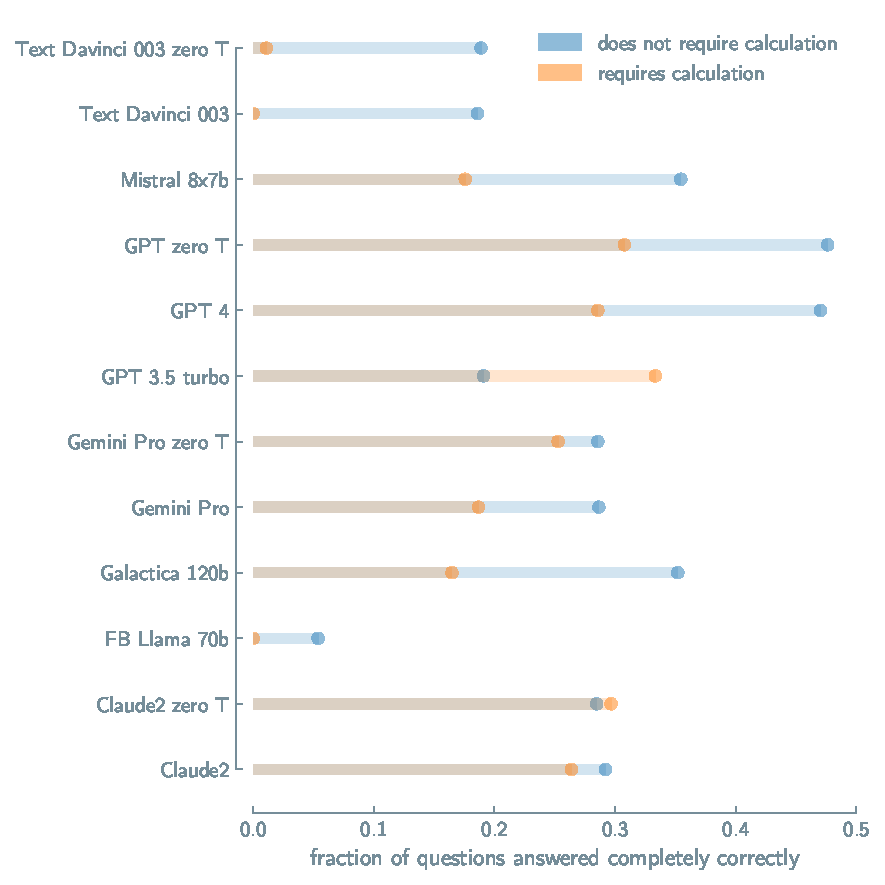
\includegraphics{figures/chem-bench-completley-correct-calculation-vs-no-calculation.pdf}
    \caption{Caption}
    \label{fig:performance_by_topic}
\end{figure}

In this spider chart, the worst score for every dimension is zero (no question answered completely correctly) and the best score is one (all questions answered correctly). 
Thus, a larger colored area indicates a better performance. 
One can observe that this performance varies widely across models and topics. 
While computational chemistry and biochemistry receive relatively high scores for many models, this is not the cases for topics such as chemical safety or analytical chemistry.
% In the subfield of analytical chemistry the prediction of the number of peaks observable in a \gls{nmr} spectrum proved difficult for the models (e.g., \variable{outputs/subset_scores/is_number_nmr_peaks_gpt-4.txt}. 
% While this question is relatively easy (\variable{outputs/human_subset_scores/is_number_nmr_peaks.txt}) for trained humans given a drawing of the compounds, models that are only shown the \gls{smiles} string of a compound have to use this to reason about the symmetry of the compound. 
% This is mirrored in the questions about point groups of compounds, which is models struggle with more than humans ().

% GFK performance -> would the models obtain a chemical license 
% Interesting twist perhaps: the performance on the university textbooks or exams is better than on the ones we automatically constructed

% Calculation vs. no calculation
Given that some of the questions in \chembench require elaborate calculations, we also analyzed if the models perform differently on those questions.
For this, we manually annotated the questions that require calculations and performed the analysis on only those questions. 

\begin{figure}
    \centering
    %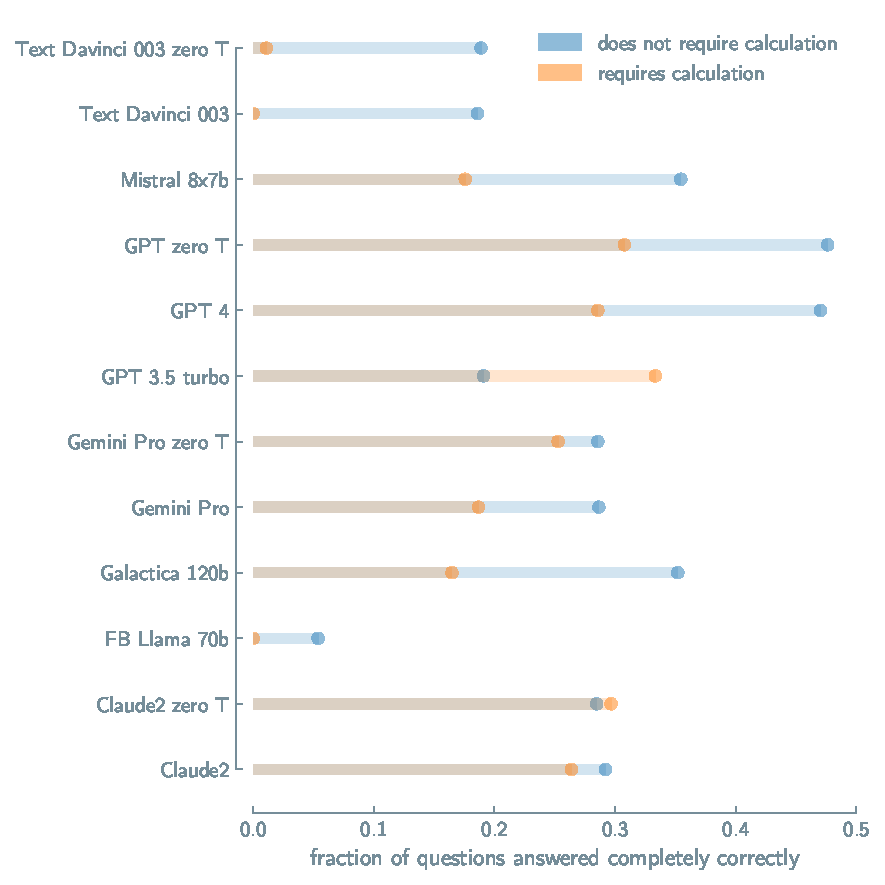
\includegraphics{figures/chem-bench-completley-correct-calculation-vs-no-calculation.pdf}
    \caption{Caption}
    \label{fig:calculation_performance}
\end{figure}

% Estimate of difficulty
One might wonder whether the models are capable of estimating if they will be able to answer a question correctly. 
If they were able to do so, incorrect answers would be less problematic as one would be able to detect when an answer is incorrect.
To investigate this, we prompted some of the top-performing models to estimate the on an ordinal scale their confidence in their ability to answer the question correctly.

\begin{figure}
    \centering
    %\includegraphics{figures/estimated_difficulty.pdf}
    \caption{Caption}
    \label{fig:estimated_difficulty}
\end{figure}

In \Cref{fig:estimated_difficulty} we show that there is no significant correlation between the estimated difficulty and whether the models answered the question correctly or not.
For applications in which humans might rely on the models to provide answers, this is a concerning observation highlighting the need for critical reasoning in the interpretation of the models' outputs.\cite{Li_2023}
For example, for the questions about the safety profile of compounds, GPT-4 reported an average confidence of XX (on a scale of 1--5) for the XX (out of XX) questions it answered in correctly (XX for the XX questions it answered correctly).

\section{Discussion and Conclusions}
Our findings also lay the groundwork for discussions for the chemical education in the future. 
Given that the models outperform the average human in our study, it is clear that we need to rethink the way we teach and examine chemistry.
Critical reasoning is increasingly important and rote solving of problems or memorization of facts is clearly a domain in which \glspl{llm} will continue to outperform humans.

% given that LLMs have parsed almost the entire internet, it is perhaps not surprising to seem them perform well on many of the task which often require 
% specific knowledge humans might not have at hand without consulting an additional knowledge bank 
% when it comes to reasoning tasks (NMR, point groups) the humans tend to beat LLMs 


% \subsection{Future work}
% - Advanced prompting techniques such as CoT and test time strategies

% - More advanced systems with chemnistry specific tools

% - More systematic human baseline: Ask people to come in, do not allow to skip questions

\section{Methods}

\subsection{Curation workflow}\label{sec:curation}
For our dataset we curated questions from existing exams, but also programmatically created new questions.
Questions were added via Pull Requests on our GitHub repository and only merged into the main collection after passing manual review.

To ensure that the questions do not enter a training dataset we use the canary string of the Big Bench project.
This requires that \Gls{llm} developers filter their training dataset for this canary string.

\begin{figure}
    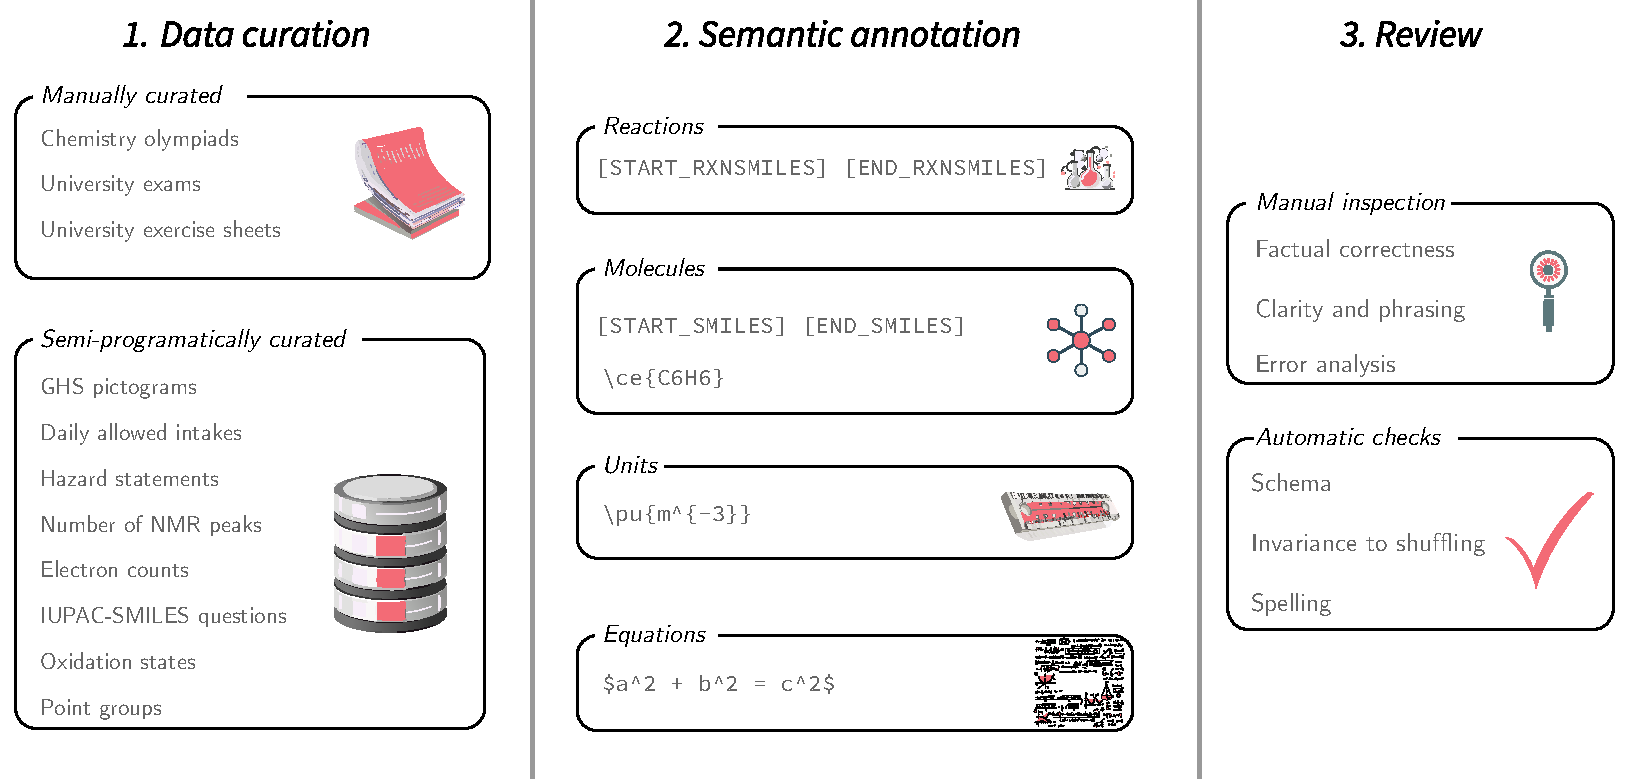
\includegraphics[width = \textwidth]{figures/chem-bench.pdf}
    \caption{\textbf{Data curation workflow}.}
\end{figure}

\paragraph{Manually curated questions}

\subparagraph{Analytical chemistry}
The \variable{output/question_count_per_dir/json_file_counts_analytical_chemistry.txt} questions are based on master student examination papers at the University of Jena (Germany). 
These questions focus on the principles and techniques employed in analytical chemistry.

\subparagraph{Combustion engineering}
These \variable{output/question_count_per_dir/json_file_counts_combustion_engineering.txt} questions are based on master student examination papers at the University of Magdeburg (Germany). 
They explore topics related to combustion processes and engineering principles.

\subparagraph{Functional materials and nanomaterials}
The \variable{output/question_count_per_dir/json_file_counts_func_mats_and_nanomats.txt}  questions are based on exercises in a seminar conducted at the University of Jena (Germany), delving into topics concerning functional materials and nanomaterials, exploring their properties and applications.

\subparagraph{General chemistry}
\variable{output/question_count_per_dir/json_file_counts_Gen_Chem_MCA.txt} questions originate from examinations for grade 10 at Marist Comprehensive Academy Uturu (Nigeria). 
They cover fundamental concepts in chemistry suitable for students at the secondary school level.
In addition, we included questions based on the general chemistry courses of the Bachelor of Science in Chemistry at the Technical University of Munich (Germany), focusing on inorganic chemistry (\variable{output/question_count_per_dir/json_file_counts_ac_faessler_tum.txt}) and principles of chemistry (\variable{output/question_count_per_dir/json_file_counts_pum_tum.txt}).

\subparagraph{International Chemical Olympiad}
\variable{output/question_count_per_dir/json_file_counts_icho.txt} questions are based on various countries' Chemical Olympiads, including those held in the USA, UK, and Moldova.

\subparagraph{Material synthesis}
\variable{output/question_count_per_dir/json_file_counts_materials_synthesis.txt} questions are based on seminars on material synthesis at the University of Jena (Germany), focusing on the methods and techniques employed in the synthesis of various materials.

\subparagraph{Organic reactivity}
\variable{output/question_count_per_dir/json_file_counts_organic_reactivity.txt}  questions are primarily sourced from tutorials and exam papers at for the Bachelor of Science in Chemistry at the Technical University of Munich (Germany), exploring reactions and mechanisms in organic chemistry.

\subparagraph{Periodic table}
\variable{output/question_count_per_dir/json_file_counts_periodic_table_properties.txt} questions are manually created to cover various aspects and trends of the periodic table.

\subparagraph{Polymer chemistry}
\variable{output/question_count_per_dir/json_file_counts_polymer_chemistry.txt} questions are based on examinations held at the University of Hamburg (Germany), covering topics related to polymer chemistry and its applications.

\subparagraph{Chemical reactivity}
\variable{output/question_count_per_dir/json_file_counts_reactive_groups.txt} questions are framed based on information from the Cameo Chemicals website (\url{https://cameochemicals.noaa.gov/reactivity}), exploring the reactivity of various chemicals and compounds.

\subparagraph{Chemical safety} 
This category comprises a total of \variable{output/question_count_per_dir/json_file_counts_safety.txt} questions, including semi-programmatically created questions covering areas such as GHS classification, hazard statements, \gls{dai}, and pictograms from the PubChem database \cite{pubchem} (see below for details). 
Additionally, it explores crucial topics like materials' compatibility (\variable{output/question_count_per_dir/json_file_counts_materials_compatibility.txt} questions) and chemical compatibility (\variable{output/question_count_per_dir/json_file_counts_chem_chem_comp.txt} questions), essential for understanding the hazardous impact of mixing certain materials and chemicals. 
Furthermore, it includes inquiries about the Federal/State Working Group on Chemical Safety (BLAC), consisting of \variable{output/question_count_per_dir/json_file_counts_blac_gfk.txt} questions. 
These questions are based on the question bank used for the expertise examination (\enquote{Sachkundeprüfung}) according to §11 of the Chemical Prohibition Ordinance (\enquote{Chemikalien-Verbotsverordnung}).
Moreover, this category addresses questions lab safety and topics such as pharmacology, toxicology, material safety data sheets, and chemical safety data sheets. 
The chemical safety category stands out as one of the primary focus areas within the \chembench corpus.

\subparagraph{NMR spectroscopy}
Questions are based on images shared via the Twitter account \url{https://twitter.com/NMRspectroscopy}, focusing choosing appropriate \gls{nmr} experiments.


\paragraph{Semi-programatically generated questions}

\subparagraph{Oxidation states}
\variable{output/question_count_per_dir/json_file_counts_oxidation_states.txt} questions regarding oxidation states are based on data from the website \url{https://www.cheminfo.org/}. 

\subparagraph{Total electron count of molecules}
\variable{output/question_count_per_dir/json_file_counts_electron_counts.txt} questions pertaining to the total electron count of molecules are based on data from the website \url{https://www.cheminfo.org/}. 
These inquiries involve determining the electron count of atoms in various chemical contexts. The calculations for these tasks are facilitated using the RDKit package \cite{rdkit}.

\subparagraph{Number of isomers}
We used MAYGEN\cite{Yirik_2021} to compute the number of isomers for a set of randomly sampled \gls{smiles} from the ZINC dataset.\cite{Irwin_2012}
To obtain the answers for false options we sampled from the set of number of isomers. In total, we generated \variable{output/question_count_per_dir/json_file_counts_number_of_isomers.txt} questions.

\subparagraph{Point group for molecules}
\variable{output/question_count_per_dir/json_file_counts_point_group.txt} questions involve predicting the point group for molecules. Our ChemCaption tool (\url{https://github.com/lamalab-org/chem-caption}) is utilized for data generation. 
Given a molecule, it uses spglib\cite{spglib} to identify the point group. 
Assigned point groups were manually verified to only include well-defined cases.

\subparagraph{SMILES-IUPAC}
We scraped pairs of \gls{smiles} and \gls{iupac} names from the PubChem database \cite{pubchem} and then framed \variable{output/question_count_per_dir/json_file_counts_smiles_to_name.txt} questions involve converting \gls{smiles} notation to \gls{iupac} nomenclature.
\variable{output/question_count_per_dir/json_file_counts_name_to_smiles.txt} questions involve the reverse task, i.e., converting \gls{iupac} nomenclature to \gls{smiles} notation.


\subparagraph{Number of NMR peaks} 
To generate the \variable{output/question_count_per_dir/json_file_counts_name_to_smiles.txt}  tasks about the number of \gls{nmr} peaks, we randomly sampled \gls{smiles} from the ZINC database\cite{Irwin_2012} and then used OpenChemLib\cite{openchemlib} to compute the number of diasterotopically distinct hydrogen atoms. 
We then sampled from the set of number of peaks (excluding the correct answer) to obtain the false answer options.

\subparagraph{GHS, hazard statements and DAI}
The \gls{ghs} classification, hazard statements and \gls{dai} data have been extracted from PubChem.\cite{pubchem}
The former two have been mined via the PubChem \gls{api}, while the latter has been manually compiled. 
In total, we generated \variable{output/question_count_per_dir/json_file_counts_pictograms.txt} questions about the \gls{ghs} classification of chemicals, \variable{output/question_count_per_dir/json_file_counts_h_statements.txt} questions about definition of hazard statements, and \variable{output/question_count_per_dir/json_file_counts_dai.txt} questions about \glspl{dai}.
The \glspl{dai} have been curated to contain only records approved by the \gls{who}.
The chemicals in this class of questions belong to one of the three classes: pesticides (e.g., calcium arsenate), insecticides (e.g., cyfluthrin) or herbicides (e.g. 2,4-D).

\subsection{Model evaluation workflow}

\paragraph{Prompting}

To maintain the consistency with the training, we employ distinct prompt templates in general tailored for completion models and instruction-tuned models. 
We pose instruction or impose constraints on the models within these templates to receive response in a specific format so that a robust, fair and consistent parsing can be performed as explained in \Cref{sec:parsing}.
Certain models are trained with special annotations and LaTeX syntax for scientific notations, chemical reactions, or symbols embedded within the text. 
For example, all the SMILES representations are encapsulated within \texttt{[START\_SMILES][\text backslash END\_SMILES]} in Galactica\cite{taylor2022galactica}.
Our prompting strategy consistently adheres to  these details in a model-specific manner by post-processing \LaTeX syntax, chemical symbols, chemical equations and physical units (by either adding or removing wrappers).



\paragraph{Parsing}
Our parsing workflow is, by default, multistep and primarily based on regular expressions.
In the case of instruction-tuned models we first attempt to identify the \texttt{[ANSWER][\textbackslash ANSWER]} environment we prompt the model to report the answer in.
In the case of completion models, this step is skipped. From there, we attempt to extract the relevant enumeration letters (for multiple-choice questions) or numbers.
In the case of numbers, our regular expression was engineered to be able to deal with various forms of scientific notation.
As initial tests indicated that models sometimes return integers in the form of words, e.g. \enquote{one} instead of \enquote{1}, we also implemented a word-to-number conversion.
In case these hard-coded parsing steps fail, we fall back to using a \gls{llm}, e.g. Claude-2, to parse the completion.
Manual verification indicates that this \gls{llm}-based parsing is not a relevant error source and has been performed correctly in all cases we checked (randomly sampled 4 questions per topic).

\paragraph{Models}
\subparagraph{Completion models}
We used \texttt{Galactica-120b}\cite{taylor2022galactica} with the default settings 


\subparagraph{Instruction-tuned models} \texttt{Claude 2} \texttt{Claude3 (Opus)}\cite{anthropicClaudeModelFamily2024}
\texttt{GPT-4}\cite{openai2024gpt4}
\texttt{GPT-3.5-turbo}\cite{brown2020language}
\texttt{Gemini Pro}\cite{gemini}
\texttt{Mixtral-8x7b}\cite{jiang2024mixtral}
\texttt{Llama2-70b}\cite{touvron2023llama}
\texttt{pplx-7b-chat}

\subparagraph{Tool augmented models}
In addition to directly prompting \glspl{llm}, we also investigated the performance of tool-augmented systems.
For this we, on the one hand, investigated the \texttt{online} model of Perplexity.AI and, on the other hand, \texttt{gpt-3.5-turbo} as well as \texttt{claude-2}, with ReAct-style tool augmentation.\cite{yao2023react}
The latter two models had access to WolframAlpha, the ArXiv \gls{api}, a Python interpreter, as well as web search (using DuckDuckGo).
We implemented the system using Langchain with the default prompts and constrained the system to a maximum of ten \gls{llm} calls.


\subsection{Confidence estimate}
To estimate the models' confidence we prompted them with the question (and answer options for \gls{mcq}) and the task to rate their confidence to produce the right answer on a scale from 1 to 5. 

\subsection{Human baseline}

\paragraph{App} To facilitate the collection of responses, we developed a responsive web application in Typescript using the Next.js\cite{nextjs} app router framework.
This application handles serving the user interface as well as exposes various \gls{rest} \glspl{api} for relevant operations.
We utilize a MySQL\cite{mysql} database and Prisma \gls{orm}\cite{prisma} for efficient database management.
The web application is styled with Tailwind CSS\cite{tailwindcss} using the shadcn/ui component library and uses NextAuth\cite{nextauth} for easy and secure user authentication and postMark for sending Emails.
The application is hosted on the Vercel web hosting platform.

\paragraph{Question selection} \label{sec:subset-selection}
Since we anticipated that we will not be able to collect enough responses for every question to allow for a meaningful statistical analysis, we decided on showing a relevant subset of all questions to the human scorers.
For selecting the subset, we decided on addressing two questions:
\begin{itemize}
    \item Are the questions for which the models scored poorly just too difficult or unanswerable?
    \item Are there areas in which the performance of humans is very different from the ones of the models?
\end{itemize}
To answer the first question we selected X questions that all \glspl{llm} (model names) from an initial scoring round did not answer correctly.
From those we picked X diverse one using greedy MaxMin sampling on the embeddings on the questions computed using BART (see below).


\paragraph{Study design}
For our initial study we wanted to maximize the response rate given our available resources. 
For this reason, we did not opt for a highly controlled study setting. 
That is, while users were prompted to not use external tools other than a calculator and to not consult with other humans, we do not have any way to verify that the participants complied with those rules. 
Note that users were also allowed to skip questions.

Another aspect of requiring unsupervised question answering is that in real life humans have tools and are able to use them for answering any question of interest. 
In our current study, we prompted users to not use those tools.

\paragraph{Participants}
Users were open to report about their experience in chemistry. 
Overall, \variable{output/num_users_with_education_info.txt} did so. 
Out of those, \variable{output/num_human_phd.txt} reported to have been awarded a Ph.D.
\variable{output/num_human_postdoc.txt} are beyond a first postdoc, \variable{output/num_human_master.txt} have a master's degree, and \variable{output/num_human_bachelor.txt} have a bachelor's degree and for \variable{output/num_human_highschool.txt} the highest awarded degree is from high school.


\paragraph{Comparison with models}
To compare the performance of humans (who might have answered only some questions) with the performance of models (which answered all questions), we focussed on questions which at least four humans answered and limited the pool of human scorers to those who answered at least 100 questions (i.e., \variable{output/num_humans_with_more_than_100_scores.txt} humans). 
The latter threshold was chosen to limit it to humans who made serious attempts at systematically answering a part of the questions. 
This analysis might lead to potential biases, most likely in favor of humans as they were allowed to skip questions. \variable{output/num_humans_with_204_scores.txt} humans answered more than 200 questions.


\subsection{Classification of questions into topics}\label{sec:meth-topic} When curating our dataset we systematically recorded keywords and sources.
To allow for analysis of the model performance as a function of the topic, we leverage this information together with sequence classification models.
For questions which can easily be assigned to a topic based on the source (e.g., number of NMR peaks, chemical compatibility, toxicology exam questions) we use this information to make the assignment.
For the remaining ones, e.g., from chemistry olympiad questions, we use zero-short sequence classification\cite{zeroshotsequence} using the BART model\cite{bart, FacebookBART}, which our preliminary analysis found to be more robust than topic modeling based on embeddings from OpenAI's \texttt{ada} model or Cohere's \texttt{Cohembed-english-v3.0} model.


\section*{Data and code availability}
The code and data for \chembench is available at \url{https://github.com/lamalab-org/chem-bench} and archived at \url{XXX}.
The code for the app for our human baseline study is available at \url{https://github.com/lamalab-org/chem-bench-app}. 
To ensure reproducibility, this manuscript was generated using the \href{https://show-your.work/en/latest/}{showyourwork!} framework.\cite{Luger2021}
The code to rebuild the paper (including code for all figures and numbers next to which there is a GitHub icon) can be found at \url{https://github.com/lamalab-org/chembench-paper}. 
To facilitate reproduction, some intermediate results of the analysis are cached at \url{http://dx.doi.org/10.5072/zenodo.34706}.

\section*{Acknowledgements}
This work was supported by the Carl Zeiss Foundation and a \enquote{Talent Fund} of the \enquote{Life} profile line of the Friedrich Schiller University Jena.
We also want to acknowledge access to the HPC cluster of Stability.AI.
M.A. expresses gratitude to the European Research Council (ERC) for evaluating the project with the reference number 101106377 titled ‘‘CLARIFIER’’ and accepting it for funding under the HORIZON TMA MSCA Postdoctoral Fellowships - European Fellowships. 
Furthermore, M.A. acknowledges the funding provided by UK Research and Innovation (UKRI) under the UK government’s Horizon Europe funding guarantee (Grant Reference: EP/Y023447/1; Organization Reference: 101106377).


\section*{Conflicts of interest}
K.M.J.\ is a paid consultant for OpenAI. M.P.\ is employee of Stability.ai and A.M.\ and N.A.\ are paid contractors of Stability.AI.

\section*{Author contributions}

\footnotesize
\insertcredits
\normalsize



\appendix
\section{Appendix}

\subsection{Desired properties of a chemistry benchmark} \label{sec:desired-properties}

\begin{itemize}
    \item \emph{End-to-end automation}. For model development, the evaluations must be run many times (e.g., on regular intervals of a training run).
    Approaches that rely on humans scoring the answers of a system\autocite{Schulze_Balhorn_2024, ai4science2023impact, castro2023large} can thus not be used.
    \item \emph{Careful validation by experts}. Manual curation is needed to minimize the number of incorrect or unanswerable questions.\autocite{northcutt2021pervasive}
    This is motivated by the observation that many widely used benchmarks are plagued by noisiness.\autocite{Frye_2023, Awg}
    \item \emph{Usable with models that support special treatment of molecules}. Some models, such as Galactica\autocite{taylor2022galactica}, use special tokenization or encoding procedures for molecules or equations.
    The benchmark system must encode the semantic meaning of various parts of the question or answer to support this.
    \item \emph{Usable with black box systems}. Many relevant systems do not provide access to model weights or raw logits.
    This might be the case because the systems are proprietary or because they involve not only \glspl{llm} but also external tools such as search \glspl{api} or code executors.\autocite{schick2024toolformer, karpas2022mrkl, yao2022react}
    Thus, a benchmark should not assume access to the raw model outputs but be able to operate on text completions.
    \item \emph{Probing capabilities beyond answering of \glspl{mcq}}. In real-world chemistry, as well as higher-level university education, multiple-choice questions are seldom utilized.
    Yet, most benchmarking frameworks focus on the \gls{mcq} setting because of the ease of evaluation. Realistic evaluations must measure capabilities beyond answering \gls{mcq}.
    \item \emph{Cover a diverse set of topics}. Chemistry, as the \enquote{central science}, bridges multiple disciplines.\autocite{Aspuru_Guzik_2018} To even just approximate \enquote{chemistry capabilities} the topics covered by a chemistry benchmark must be very diverse.
    \item \emph{Cover diverse skills}. To holistically judge performance it is important to cover questions relying on reasoning, calculation, knowledge, and intuition.
    \item \emph{Cover a range of difficulty levels}. To allow for a continuous measure of improvement for a range of different (evolving) systems, a benchmark should cover a wide range of difficulty levels.
    \item \emph{Impossible to completely solve with current models}. A benchmark should contain questions that are impossible to solve with current models. If current models can solve all questions, the benchmark provides no useful signal.
\end{itemize}

\subsection{Related work}
Existing benchmarks such as those from \textcite{guo2023large}, \textcite{sun2023scieval}, \textcite{Schulze_Balhorn_2024}, \textcite{Cai_2024} fail to comply with most of the requirements stipulated above.
While these benchmarks could provide valuable insights in the short term, they cannot follow the rapid additions to the \gls{llm} space.
\chembench aims to correct this through a set of developments: compatibility with BigBench, end-to-end automation, a particular focus on chemical safety, employment of diverse prompting strategies, and specialized notation for molecules and mathematical symbols.
Moreover, our robust framework, including the platform \url{chembench.org}, will engage the community in open-source contributions.

\clearpage
\subsection{Benchmark corpus}
To ensure maximal interoperability with existing benchmarks or tools, we curated the data in an extended form of the widely used BigBench format.\autocite{srivastava2022beyond}
This also implies that future baselines can be built on top of our infrastructure if saved in the same format.

\subsubsection{Curation workflow}
Questions were added via pull requests to the \chembench repository on GitHub.
This allowed for a manual review of each question by expert reviewers (with backgrounds in chemistry, materials science, chemical engineering, and physics).
The reviews were conducted directly on the GitHub platform, where our entire curation history is also publicly available.

The general guidelines followed by the reviewer are the following:

\begin{itemize}
    \item \textbf{Originality:} Questions should not be readily findable online or in other easily accessible sources (example \url{https://github.com/lamalab-org/chem-bench/pull/392#discussion_r1694299474})
    \item \textbf{Ambiguity:} Questions with unclear wording or multiple interpretations (example \url{https://github.com/lamalab-org/chem-bench/pull/420#discussion_r1698147159} )
    \item \textbf{Factual or heuristic Errors: }Questions containing factual inaccuracies or misconceptions are not included (example \url{https://github.com/lamalab-org/chem-bench/pull/389#discussion_r1686187301})
    \item \textbf{Out of Scope:} Questions outside the realm of chemistry are rejected.
    \item \textbf{Clarity and Difficulty: } They should pose a challenge and encourage exploration within the chemical domain.
    \item \textbf{Contribution to Dataset Diversity: }Questions should cover a wide range of chemical concepts and sub-disciplines. They should add value by expanding the breadth of the dataset. That is, questions already multiple (>10) times in the corpus in a similar form are rejected.
\end{itemize}

Reviewers also solved the questions to verify the answers. They also performed web searches to ensure questions were not easily found online. The reviewers often guided the revision process to ensure the question aligned with the guidelines. Questions that don't meet the criteria are either rejected or suggested for revision and most often, they are modified to a new question. Reviewers also provide feedback on the skill and difficulty annotations.

In addition to the manual review, we also performed automated checks to ensure the quality of the questions. The schemas, Latex templating, and other formatting aspects are checked automatically using GitHub Actions.

\subsubsection{Composition}

\Cref{fig:cb_humanset} shows the distribution of topics and required skills in the human subset of the \chembench corpus.

\begin{figure}
    \centering
    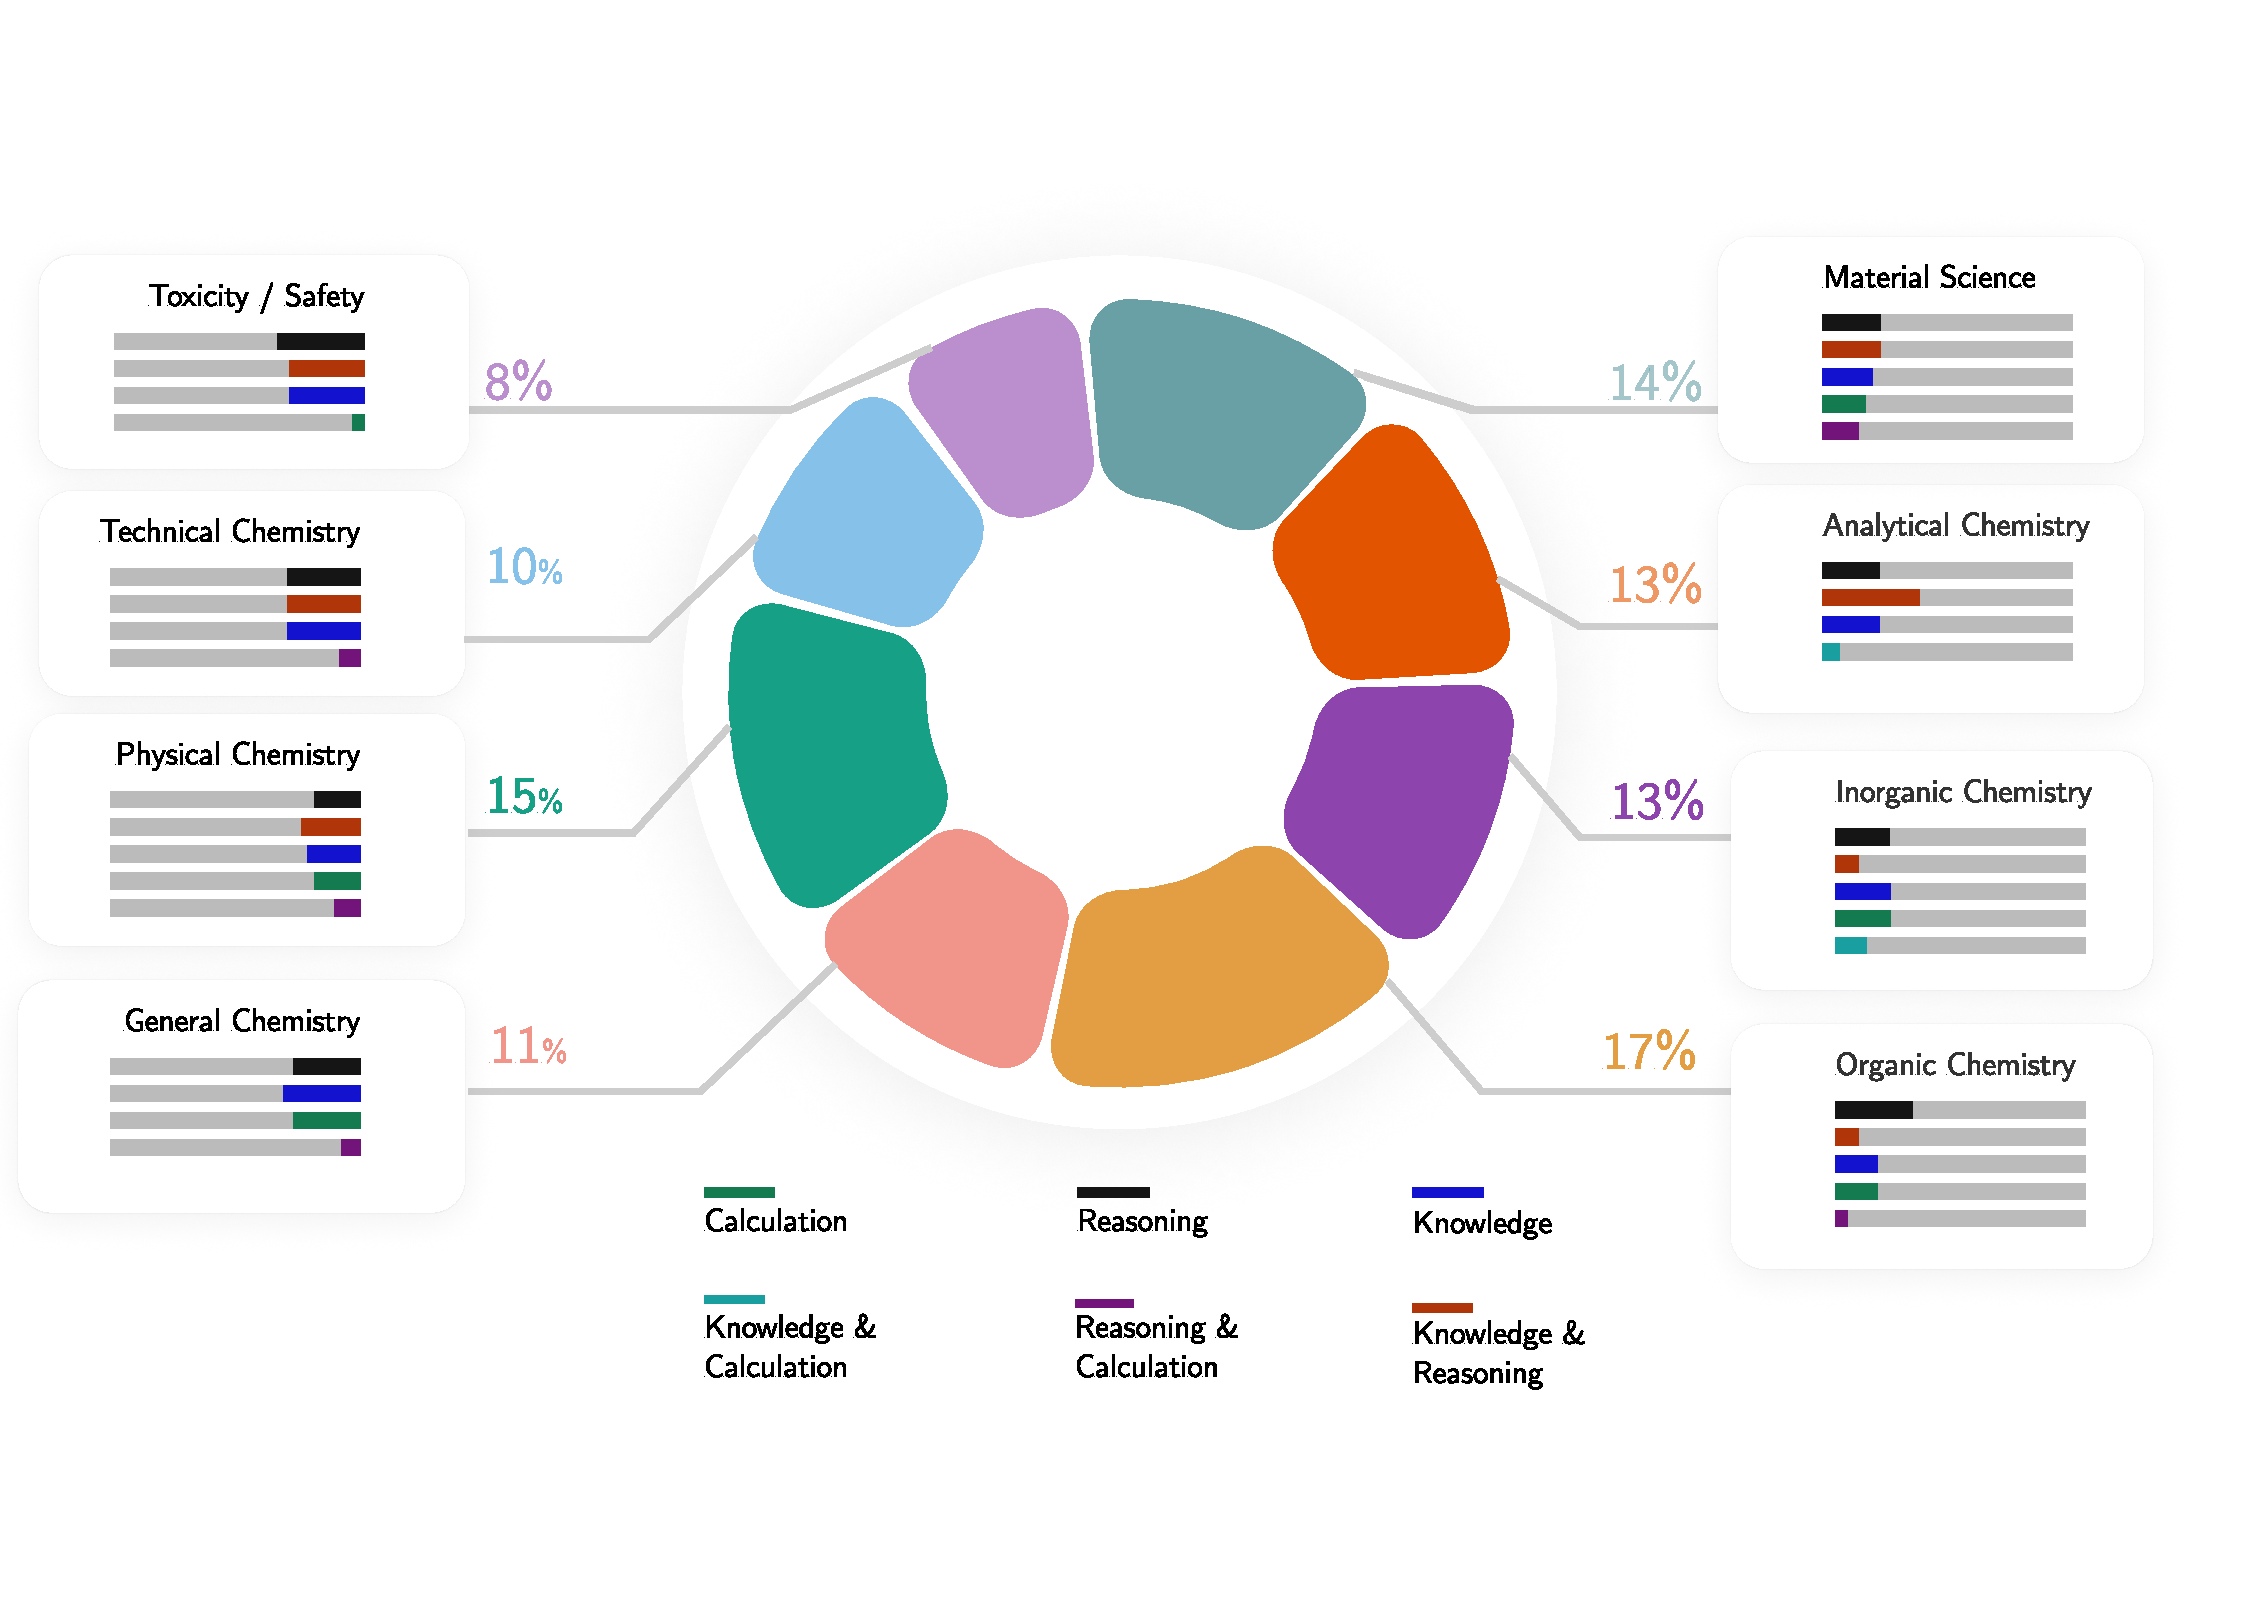
\includegraphics[width=\textwidth]{figures/CB_HUMANSET_FIG_V1.pdf}
    \caption{\textbf{Composition of the human subset.} The circular plot shows the distribution of topics and required skills in the human subset of the \chembench corpus. The human subset is a representative subset of the full corpus, with a balanced distribution of topics and skills.}
    \label{fig:cb_humanset}
\end{figure}

The corpus of the questions in \chembench, as shown in \Cref{tab:chembench_corpus_topic}, can be divided according to which chemical topic they belong to.

%\begin{table}
%    \centering
%    \small
%    \caption{\textbf{Examples for each of the topics considered in the evaluation of the \chembench corpus.} The table shows the percentage of questions in the corpus that belong to each topic, as well as example questions.}
%    \label{tab:chembench_corpus_topic}
%    {\fontsize{8}{9}\selectfont
%        \begin{tabularx}{\textwidth}{X}
%            \toprule
%            \multicolumn{1}{c}{\textbf{Analytical Chemistry} 166 Questions (5.8\%)} \\
%            \midrule
%            Which of the following analytical methods is most appropriate for performing a survey analysis of a solid sample containing various metals? \\
%            A. X-ray fluorescence analysis \\
%            B. Differential pulse polarography \\
%            C. Flame-atomic absorption spectroscopy \\
%            D. Gas chromatography with flame ionization detector \\
%            E. Hydride generation atomic absorption spectroscopy \\
%            \midrule
%            \multicolumn{1}{c}{\textbf{Chemical Preference} 1001 Questions (35\%)} \\
%            \midrule
%            Imagine an early virtual screening campaign setting (accounting for simple aspects such as oral availability and small molecular profile, but no other modalities such as covalency or bifunctionality). Which of the following two candidates would you prefer for further development? \\
%            [START\_SMILES]N\#Cc1ccc(OCCCN2CC3CN\-(CCNS(=O)(=O)c4ccc(F)cc4)CC(C2)O3)cc1\-[END\-\_SMILES] \\
%            [START\_SMILES]O=C1CC(c2ccc(CC(NS(=O)\-(=O)\-c3cc(Cl)cc(Cl)c3)c3nc4ccccc4[nH]3)cc2)S\-(=O)\-(=O)N1[END\_SMILES] \\
%            \midrule
%            \multicolumn{1}{c}{\textbf{General Chemistry} 152 Questions (5.3\%)} \\
%            \midrule
%            Which of the following salts is an acidic salt? \\
%            A. \ce{NH4Cl} \\
%            B. \ce{Na2CO3} \\
%            C. \ce{NaH2PO4} \\
%            D. \ce{Zn(OH)Cl} \\
%            \midrule
%            \multicolumn{1}{c}{\textbf{Inorganic Chemistry} 94 Questions (3.3\%)} \\
%            \midrule
%            What is the oxidation number of the metal in the compound \ce{[ZrF7]^{3-}}\\
%            \midrule
%            \multicolumn{1}{c}{\textbf{Materials Science} 89 Questions (3.1\%)} \\
%            \midrule
%            For NMR analysis, you need to digest the MOF in a strong acid to remove the linker and leave the metal clusters intact. Why would one choose \ce{HF} over \ce{HCl} for this purpose? \\
%            A. \ce{F-} forms a stable bonds to the metal ions \\
%            B. \ce{HF} has a better water solubility than \ce{HCl} \\
%            C. \ce{HF} has a higher boiling point than \ce{HCl} \\
%            D. \ce{HF} is a weaker acid than \ce{HCl} \\
%            \midrule
%            \multicolumn{1}{c}{\textbf{Organic Chemistry} 441 Questions (15.5\%)} \\
%            \midrule
%            What is the reaction mechanism that describes the following reaction (represented using reaction SMILES) [START\_RXNSMILES]CCCl.CO[Na]>>[Na]Cl.CCOC\-[END\_RXNSMILES]? \\
%            A. $E_1$ \\
%            B. $E_{cb}$ \\
%            C. $S_N1$ \\
%            D. $S_N2$ \\
%            \midrule
%            \multicolumn{1}{c}{\textbf{Physical Chemistry} 179 Questions (6.3\%)} \\
%            \midrule
%            The Born-Oppenheimer (BO) approximation is widely used in computational chemistry, but its accuracy can vary depending on the system. Among the following options, for which system is the Born-Oppenheimer approximation likely to be least applicable? \\
%            A. \ce{C60} \\
%            B. \ce{CH4} \\
%            C. \ce{Fe(CO)5} \\
%            D. \ce{H2+} \\
%            E. \ce{NaCl} \\
%            \midrule
%            \multicolumn{1}{c}{\textbf{Technical Chemistry} 42 Questions (1.5\%)} \\
%            \midrule
%            Which of the following statements is true about the different types of ideal reactors? \\
%            A. In a batch reactor, the composition is uniformly mixed and remains the same throughout the reactor and at the exit \\
%            B. In a batch reactor, the fluid passes through the reactor with no mixing of earlier and later entering fluid \\
%            C. In a mixed flow reactor, the composition changes with time but is uniform everywhere within the reactor \\
%            D. In a plug flow reactor, the fluid moves in single flow through the reactor with no mixing and no overtaking \\
%            \midrule
%            \multicolumn{1}{c}{\textbf{Toxicity/Safety} 690 Questions (24.2\%)} \\
%            \midrule
%            Pindolol and propranolol are (relatively nonselective) antagonists at $\beta_1$- and $\beta_2$-adrenoceptors. However, pindolol is a partial agonist, whereas propranolol is a pure antagonist. What follows from this? \\
%            A. Pindolol has a greater therapeutic range than propranolol \\
%            B. Pindolol has a longer half-life than propranolol \\
%            C. Pindolol has intrinsic activity \\
%            D. Pindolol is more lipophilic than propranolol \\
%            E. Pindolol is more potent than propranolol \\
%            \bottomrule
%        \end{tabularx}
%    }
%\end{table}

\normalsize


In addition, as shown in \Cref{tab:cb_skillset} the \chembench corpus can be divided considering the different skills needed to solve the questions. The plot shows a balanced distribution of the required skills in the \chembench corpus. \Cref{tab:cb_skillset} shows an example question for each skill category.

\begin{figure}
    \centering
    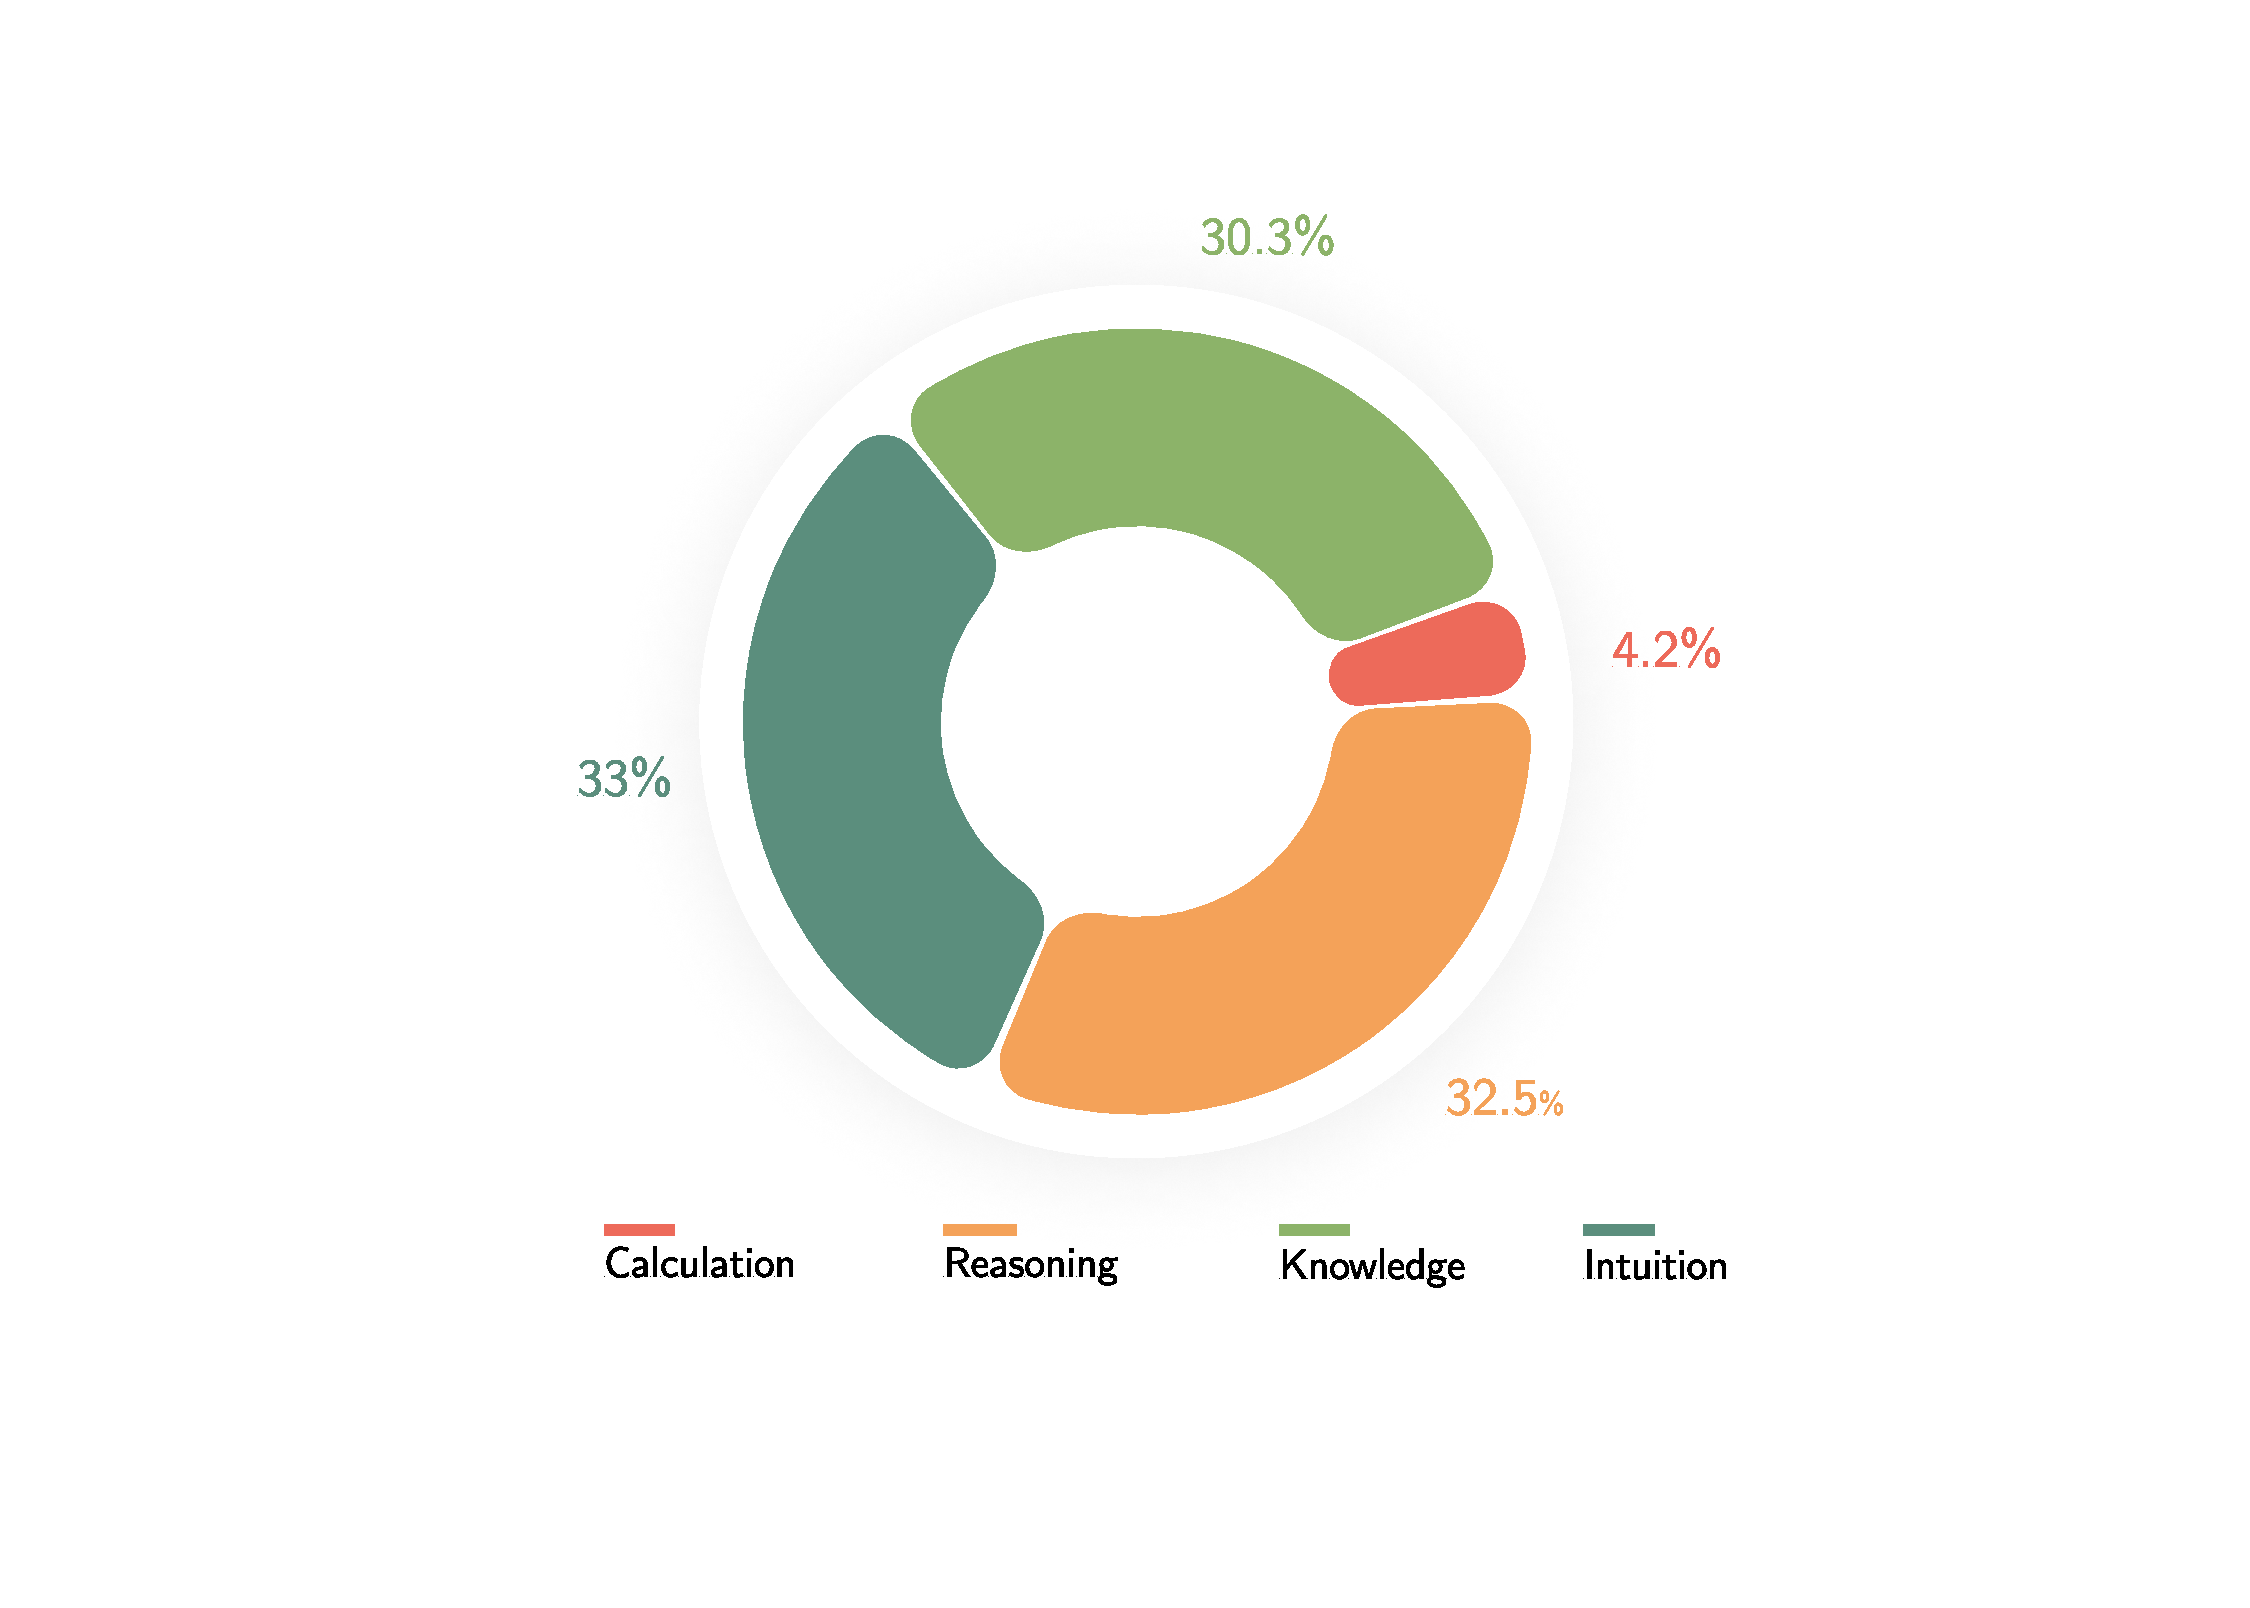
\includegraphics[width=\textwidth]{figures/CB_SKILL_FIG_V1.pdf}
    \caption{\textbf{Composition of the required skills considered in the \chembench corpus.} The circular plot shows the distribution of required skills in the \chembench corpus.}
    \label{fig:cb_skillset}
\end{figure}


\begin{table}
    \centering
    \small
    \caption{\textbf{Examples for each of the required skills considered in the \chembench corpus.} The table shows the number of questions for each skill and an example question. Note that the total count in this table is bigger than the \chembench corpus. This is because the same question can be annotated with two different \enquote{requires} skills, i.e. Reasoning and Calculation.}
    \label{tab:chembench_corpus_cognitive}
    {\fontsize{8}{9}\selectfont
        \begin{tabularx}{\textwidth}{X}
            \toprule
            \multicolumn{1}{c}{\textbf{Knowledge} 919 Questions} \\
            \midrule
            Which of the following salts is an acidic salt? \\
            A. \ce{NH4Cl} \\
            B. \ce{Na2CO3} \\
            C. \ce{NaH2PO4} \\
            D. \ce{Zn(OH)Cl} \\
            \midrule
            \multicolumn{1}{c}{\textbf{Reasoning} 987 Questions} \\
            \midrule
            How can the optical impact of quantum confinement on the electronic structure of a quantum dot be observed experimentally? \\
            A. By atomic force microscopy \\
            B. By transform infrared spectroscopy \\
            C. By measuring a photoluminescence spectrum \\
            D. By absorption spectroscopy \\
            \midrule
            \multicolumn{1}{c}{\textbf{Intuition} 1001 Questions} \\
            \midrule
            Imagine an early virtual screening campaign setting (accounting for simple aspects such as oral availability and small molecular profile, but no other modalities such as covalency or bifunctionality). Which of the following two candidates would you prefer for further development? \\
            A. [START\_SMILES]CC1(C)Oc2ccc([N+](=O)[O-])cc2[C@@H](N2CCOCC2)[C\@\@H]1O[END\_SMILES] \\
            B. [START\_SMILES]Cc1ccccc1N=C(S)N1CCC(NC\-(=O)c2ccco2)CC1[END\_SMILES] \\
            \midrule
            \multicolumn{1}{c}{\textbf{Calculation} 128 Questions} \\
            \midrule
            Given that the average molar mass of the polymer chains in this sample of poly(lactic acid) (PLA) is \SI{595}{g mol^{-1}} using end-group analysis, where \SI{0.1619}{g} of PLA was dissolved in \SI{25}{cm^3} of benzyl alcohol and titrated with \SI{0.0400}{mol dm^{-3}} \ce{KOH} solution. The volume of \ce{KOH} solution required to reach the endpoint was \SI{6.81}{cm^3}. What is the average number of monomer units in each polymer chain of this sample? \\
            \bottomrule
        \end{tabularx}
    }
\end{table}

\normalsize

In analyzing the performance of state-of-the-art models on the ChemBench corpus, we identified several chemical topics where the models consistently struggled to provide correct answers. The following table \cref{tab:chembench_corpus_models_failed_topic} presents examples of challenging questions across different chemical domains, highlighting specific areas where current models need improvement

%\begin{table}
%    \centering
%    \small
%    \caption{\textbf{Examples of topics evaluated in the \chembench corpus that the state-of-the-art model failed to answer correctly.} The table displays the percentage of questions in the corpus for each topic, along with example questions and the percentage of questions that were not answered correctly by the models.}
%    \label{tab:chembench_corpus_models_failed_topic}
%    {\fontsize{8}{9}\selectfont
%        \begin{tabularx}{\textwidth}{X}
%            \toprule
%            \multicolumn{1}{c}{\textbf{Analytical Questions} 166 Questions (5.8\%) (26.5\%)} \\
%            \midrule
%            Which of the following methods can be used to support the structure elucidation of planar molecules by examining the topography of individual molecules? \\
%            A. DESI-mass spectrometry \\
%            B. XPS \\
%            C. atomic force microscopy \\
%            D. scanning tunneling microscopy \\
%            E. secondary ion mass spectrometry \\
%            \midrule
%            \multicolumn{1}{c}{\textbf{Chemical Preference} 1001 Questions (35\%) (8.5\%)} \\
%            \midrule
%            Imagine an early virtual screening campaign setting (accounting for simple aspects such as oral availability and small molecular profile, but no other modalities such as covalency or bifunctionality). Which of the following two candidates would you prefer for further development? \\
%            [START\_SMILES]N\#Cc1ccc(OCCCN2CC3CN\-(CCNS(=O)(=O)c4ccc(F)cc4)CC(C2)O3)cc1\-[END\-\_SMILES] \\
%            [START\_SMILES]O=C1CC(c2ccc(CC(NS(=O)\-(=O)\-c3cc(Cl)cc(Cl)c3)c3nc4ccccc4[nH]3)cc2)S\-(=O)\-(=O)N1[END\_SMILES] \\
%            \midrule
%            \multicolumn{1}{c}{\textbf{General Chemistry} 152 Questions (5.3\%) (3.2\%)} \\
%            \midrule
%            Why \ce{SCl6} does not exist if other similar molecules such as \ce{SF6} exist? \\
%            A. \ce{SCl6} does not exist because of steric effects \\
%            B. \ce{SCl6} does not exist because of the high electronegativity of chlorine \\
%            C. \ce{SCl6} does not exist because of the high ionization potential of the chlorine \\
%            D. \ce{SF6} exist because of the high electronegativity of fluorine \\
%            \midrule
%            \multicolumn{1}{c}{\textbf{Inorganic Chemistry} 94 Questions (3.3\%) (4.2\%)} \\
%            \midrule
%            What is the spin-only magnetic moment (in units of Bohr-magnetons) for the low-spin case of the metal complex \ce{RhCl(CO)(PPh3)2}?\\
%            \midrule
%            \multicolumn{1}{c}{\textbf{Materials Science} 89 Questions (3.1\%) (0.9\%)} \\
%            \midrule
%            What are the conditions for the observation of effects of quantum confinement in quantum dots? \\
%            A. All dimension of the material must be smaller than exciton Bohr radius \\
%            B. One dimension of the quantum dot must be smaller than exciton Bohr radius \\
%            C. The movement od charge carriers is limited in all spatial dimensions \\
%            \midrule
%            \multicolumn{1}{c}{\textbf{Organic Chemistry} 441 Questions (15.5\%) (0.5\%)} \\
%            \midrule
%            What makes acrylates more reactive than typical hydrocarbons? \\
%            A. The carbonyl group \\
%            B. The double bond \\
%            C. The hydroxyl group \\
%            D. The vinyl group \\
%            \midrule
%            \multicolumn{1}{c}{\textbf{Physical Chemistry} 179 Questions (6.3\%) (13.4\%)} \\
%            \midrule
%            Why are polar molecules more soluble in water than non-polar molecules? \\
%            A. Non-polar molecules should break hydrogen bonds in water to dissolve \\
%            B. The entropy of the system increases when non-polar molecules dissolve in water \\
%            C. Water has a dipole and can easier isolate polar molecules from each other \\
%            D. Water makes stable dipole-dipole interactions with polar molecules \\
%            \midrule
%            \multicolumn{1}{c}{\textbf{Technical Chemistry} 42 Questions (1.5\%) (4.7\%)} \\
%            \midrule
%            Which of the following statements is/are true about granulation shaping of solid catalysts? \\
%            A. Broader product diameter distribution than pellets or extrudates \\
%            B. Facilitates reactor upscaling \\
%            C. It is also called snow-ball \\
%            D. Not suitable to prepare egg-shell catalysts \\
%            \midrule
%            \multicolumn{1}{c}{\textbf{Toxicity/Safety} 690 Questions (24.2\%) (40.4\%)} \\
%            \midrule
%            What determines the flammability of polyols? \\
%            A. Their chemical structure \\
%            B. Their low volatility \\
%            C. Their odor threshold \\
%            D. Their reaction with acids \\
%            \bottomrule
%        \end{tabularx}
%    }
%\end{table}

\normalsize

To better understand the cognitive demands of chemical assessment, we categorized the questions in the ChemBench corpus according to the primary skills required to solve them. The table \Cref{tab:chembench_corpus_models_failed_cognitive} below shows representative examples of questions that state-of-the-art models failed to answer correctly across different cognitive skill categories, including knowledge, reasoning and intuition.
\begin{table}
    \centering
    \small
    \caption{\textbf{Examples of required skills evaluated in the \chembench corpus that the state-of-the-art model failed to answer correctly} The table displays the number of questions for each skill, along with an example question that the model failed to answer.}
    \label{tab:chembench_corpus_models_failed_cognitive}
    {\fontsize{8}{9}\selectfont
        \begin{tabularx}{\textwidth}{X}
            \toprule
            \multicolumn{1}{c}{\textbf{Knowledge} 919 Questions} \\
            \midrule
            Which of the following are true for phosphoric acid? \\
            A. Is a weak acid, so it is not toxic \\
            B. Should never be tasted \\
            C. Though a component of soft drinks, reacts vigorously with water when in concentrated form \\
            \midrule
            \multicolumn{1}{c}{\textbf{Reasoning} 987 Questions} \\
            \midrule
            Which of the following elements has the largest atomic radius? \\
            A. \ce{Fr} \\
            B. \ce{He} \\
            C. \ce{Li} \\
            D. \ce{Rb} \\
            \midrule
            \multicolumn{1}{c}{\textbf{Intuition} 1001 Questions} \\
            \midrule
            Imagine an early virtual screening campaign setting (accounting for simple aspects such as oral availability and small molecular profile, but no other modalities such as covalency or bifunctionality). Which of the following two candidates would you prefer for further development? \\
            A. [START_SMILES]CCc1c(CCOC)nn(-c2ccccc2)c1-c1ccccc1[END_SMILES] \\
            B. [START_SMILES]Cc1cc(/C=C2\\C(=N)N3N=C(S(C)(=O)=O)SC3=NC2=O)c(C)n1Cc1ccccc1[END_SMILES] \\
            \midrule
            \multicolumn{1}{c}{\textbf{Calculation} 128 Questions} \\
            \midrule
            The cell potential for the overall cell reaction during electrolysis of water, \ce{2H2O(l) -> 2H2(g) + O2(g)} is \SI{-1.23 V}. What is the standard electrode potential for the half reaction, \ce{2H2O(l) -> O2(g) + 4H+(aq) + 4e-} in V? \\
            \bottomrule
        \end{tabularx}
    }
\end{table}

\normalsize




\clearpage
\subsection{Model performance} \label{sec:model_performance_app}
We also evaluated the model performance on the entire \chembench corpus.
\Cref{fig:barplot_all_correct_all_questions} shows the fraction of questions that were answered correctly by the models.

\begin{figure}[htb]
    \centering
    \includegraphics{figures/overall_performance.pdf}
    \caption{\textbf{Overall performance of the models on the \chembench corpus.} The bar plot shows the fraction of questions that were answered completely correctly by the models. Scores computed on the entire \chembench corpus.}
    \label{fig:barplot_all_correct_all_questions}
    \script{plot_overview_performance_plot.py}
\end{figure}

\Cref{fig:all_questions_models_completely_correct_radar_overall} shows the performance of the models on the different topics of the \chembench corpus.
The general pattern of performance varies significantly between the different topics and is also observed when the models are evaluated on the entire corpus.
However, since some subjects are composed of questions from different sources, the ranking of the models is, in some instances, different from the one on \chembenchmini.

\begin{figure}[htb]
    \centering
    \includegraphics[width=\textwidth]{figures/all_questions_models_completely_correct_radar_overall.pdf}
    \caption{\textbf{Performance of the models on the different topics of the \chembench corpus.} The radar plot shows the performance of the models on the different topics of the \chembench corpus. The performance is measured as the fraction of questions answered completely correctly by the models.
    A score of 1 (full coverage until the outer line of this plot) indicates that all questions were answered completely correctly, while a score of 0 indicates that none were answered completely correctly.
    }
    \label{fig:all_questions_models_completely_correct_radar_overall}
    \script{analyze_model_reports.py}
\end{figure}




To further investigate the performance of the models, we also compared the performance on different data sources.
Compared to topics, this is a more fine-grained analysis, as topics can be composed of questions from different sources.
In \Cref{fig:performance_per_topic}, we see that the performance of the models varies significantly between the different data sources.
Interestingly, the performance of the models on questions sourced based on textbooks seems to be better for our models than some semi-programmatically created tasks, such as questions about the number of signals in an \gls{nmr} spectrum.


\begin{figure}[htb]
    \centering
    \includegraphics{figures/performance_per_topic.pdf}
    \caption{\textbf{Fraction of correctly answered questions per data source.} The heatmap shows, in color, the fraction of questions answered correctly by different systems for some of our data sources. The performance is measured as the fraction of questions answered completely correctly by the models. A score of one (red) indicates that all questions were answered completely correctly, while a score of zero (blue) indicates that none of the questions were answered completely correctly.
        We see that the performance of the models varies significantly between the different data sources. For instance, it is interesting to observe that questions sourced based on textbooks seem easier for our leading models than for humans. However, this performance does not correlate with performance on other sources, e.g., semi-programmatically created tasks such as questions about the number of signals in an \gls{nmr} spectrum.
    }
    \label{fig:performance_per_topic}
    \script{analyze_performance_per_source.py}
\end{figure}

\Cref{fig:performance_per_topic_tiny} shows the same analysis on \chembenchmini.

\Cref{fig:performance_corpus_and_tiny} shows the performance of the models on the \chembench corpus and the \chembenchmini subset. The relative performance difference between both is quite similar across most models.
This makes \chembenchmini subset a reliable subset for human baseline comparison and particularly valuable for rapid prototyping and initial model assessment phases.

An interesting observation is the significant impact of chemical preference tasks on \GPTFour's scores. A detailed breakdown of overall accuracy into scores on different skills and difficulty levels is provided in \Cref{table:performance_table} and \Cref{tab:performance_table_human_subset} for \chembench corpus and the \chembenchmini subset, respectively.


\begin{figure}[htb]
    \centering
    \includegraphics{figures/performance_per_topic_tiny.pdf}
    \caption{\textbf{Fraction of  correctly answered questions per data source on \chembenchmini.} The heatmap shows, in color, the fraction of questions answered completely correctly by different systems for some of our data sources. The performance is measured as the fraction of questions answered completely correctly by the models. A score of one (red) indicates that all questions were answered completely correctly, while a score of zero (blue) indicates that none were answered completely correctly.
        We see that the performance of the models varies significantly between the different data sources. For instance, it is interesting to observe that questions sourced based on textbooks seem easier for the leading models than for humans. However, this performance does not correlate with performance on other sources, e.g., semi-programmatically created tasks such as questions about the number of signals in an \gls{nmr} spectrum.
    }
    \label{fig:performance_per_topic_tiny}
    \script{analyze_performance_per_source.py}
\end{figure}


\begin{figure}[htb]
    \centering
    \includegraphics{figures/corpus_human_comparison.pdf}
    \caption{\textbf{
        Performance of the models on the \chembench corpus and \chembenchmini subset.} The bar plot shows the fraction of questions that were answered completely correctly, highlighting the relative performance of different models on both the \chembench corpus and the \chembenchmini subset.
        We see that the model ranking remains fairly consistent across both sets}
    \label{fig:performance_corpus_and_tiny}
    \script{corpus_humanset_performance.py}
\end{figure}

\begin{table}
    \caption{\textbf{Performance of the models on the \chembench corpus.} The table shows the fraction of questions answered completely correctly by the models for different skills and difficulty levels.}
    \resizebox{\textwidth}{!}{
    \variable{output/performance_table.tex}
    }
    \label{tab:performance_table}
\end{table}

\begin{table}
    \caption{\textbf{Performance of the models on \chembenchmini.} The table shows the fraction of questions answered completely correctly by the models for different skills and difficulty levels.}
    \resizebox{\textwidth}{!}{
    \variable{output/performance_table_human_subset.tex}
    }
    \label{tab:performance_table_human_subset}
\end{table}



\clearpage

\subsection{Performance as a function of molecular features} \label{sec:molecular_features}
To better understand if the performance of the models is correlated with specific features of the molecules, we analyzed the performance of the models as a function of the number of atoms and the complexity of the molecules.
\Cref{fig:correlation_plot_is_number_nmr_peaks_complexity} shows that the performance of the models is not correlated with the complexity of the molecules but rather with the number of atoms (\Cref{fig:correlation_plot_is_number_nmr_peaks_num_atoms}, similar trivial correlation for \Cref{fig:correlation_plot_is_electron_counts_num_atoms}).
%The corresponding Spearman correlation coefficients are listed in \Cref{tab:correlation_coefficients}.

\begin{figure}[!h]
    \centering
    \includegraphics[width=\textwidth]{figures/correlation_plot_is_number_nmr_peaks_complexity.pdf}
    \caption{\textbf{Dependence of the mean absolute error in predicting the number of NMR signals on the Böttcher complexity of the molecules.} The complexity measure proposed by \textcite{B_ttcher_2016} is an information-theoretic additive measure of compound complexity that follows chemical intuitions.
    The plot shows that for the \glspl{llm}, the predictive performance (measured as the mean absolute error in the prediction of the number of \gls{nmr} signals) is not correlated with the complexity of the molecules (that is, molecules tend to not to be able to predict the number of \gls{nmr} signals irregardless of molecular complexity). For inference based on reasoning, one would expect that the complexity of the molecule is a good predictor of the difficulty of the question.}
    \script{correlate_with_molecule_features.py}
    \label{fig:correlation_plot_is_number_nmr_peaks_complexity}
\end{figure}

\begin{figure}[!h]
    \centering
    \includegraphics[width=\textwidth]{figures/correlation_plot_is_number_nmr_peaks_num_atoms.pdf}
    \caption{\textbf{Dependence of the mean absolute error in predicting the number of NMR signals on the number of atoms.} }
    \script{correlate_with_molecule_features.py}
    \label{fig:correlation_plot_is_number_nmr_peaks_num_atoms}
\end{figure}


\begin{figure}[!h]
    \centering
    \includegraphics[width=\textwidth]{figures/correlation_plot_is_electron_counts_num_atoms.pdf}
    \caption{\textbf{Dependence of the mean absolute error in predicting total electron counts on the number of atoms.} The plot shows that for the \glspl{llm}, the predictive performance (measured as the mean absolute error in the prediction of the total electron counts) is sometimes correlated with the number of atoms in the molecule.}
    \script{correlate_with_molecule_features.py}
    \label{fig:correlation_plot_is_electron_counts_num_atoms}
\end{figure}


\clearpage
\subsection{Influence of model scale}
\Cref{fig:model_size_plot} shows the performance of the models as a function of the number of parameters in the model.
We see that the performance of the models correlates with their size for the models of the LLama-3 and Llama-3.1 herd of models.

\begin{figure}[!h]
    \centering
    \includegraphics[width=\textwidth]{figures/model_size_plot.pdf}
    \caption{\textbf{Performance of models as a function of model size.} The plot shows the performance of the models as a function of the parameter count. The performance is measured as the fraction of questions answered correctly by the models. We see that the performance of the models correlates with scale for the models of the LLama-3 and Llama-3.1 herd of models.}
    \script{performance_vs_model_size.py}
    \label{fig:model_size_plot}
\end{figure}


\clearpage
\subsection{Refusal detection}
\Glspl{llm} typically undergo refusal training to prevent harmful or undesirable outputs. As a result, models may decline to answer questions perceived as potentially adversarial prompts.
To automatically detect refusals, we use a modified regular expression reported by LLM Guard\autocite{llmguard} to detect commonly used refusal phrases.

\Cref{tab:refusal_counts_and_parsing} lists how many refusals were detected for the reponses of different models on \chembench. Overall, we find that refusals do not majorly affect the performance measured by \chembench.


\subsection{LLM Parsing} \label{sec:llm-parsing}

In our parsing workflow, we use pipelines based on regular expressions to extract the answers. In some cases, however, the answers are not directly extractable from the responses, for instance, when the model does not follow the formatting instructions. In these cases, we use a fallback mechanism to extract the answers. The fallback mechanism uses an \gls{llm} to extract the answers from the responses. The \gls{llm} is provided with the response and the question and is prompted to only extract but not generate the answer. We used \LlamaThreeSeventyBInstruct, accessed via the Groq API.
\Cref{tab:refusal_counts_and_parsing} tabulates the number of times the fallback mechanism was used for each model.


\begin{table}
    \centering
    \caption{\textbf{Refusal counts and parsing.} The table shows the number of refusals detected and the number of times the \gls{llm} fallback parsing mechanism was used for each model.}
    \variable{output/model_refusal_table.tex}
    \label{tab:refusal_counts_and_parsing}
\end{table}

\clearpage
\subsection{Implementation}
An overview of the benchmarking pipeline implemented in \chembench is shown in \Cref{fig:process}. More detailed information can be found in the online documentation of the \chembench package at \url{https://lamalab-org.github.io/chem-bench/}.
\begin{figure}
    \centering
    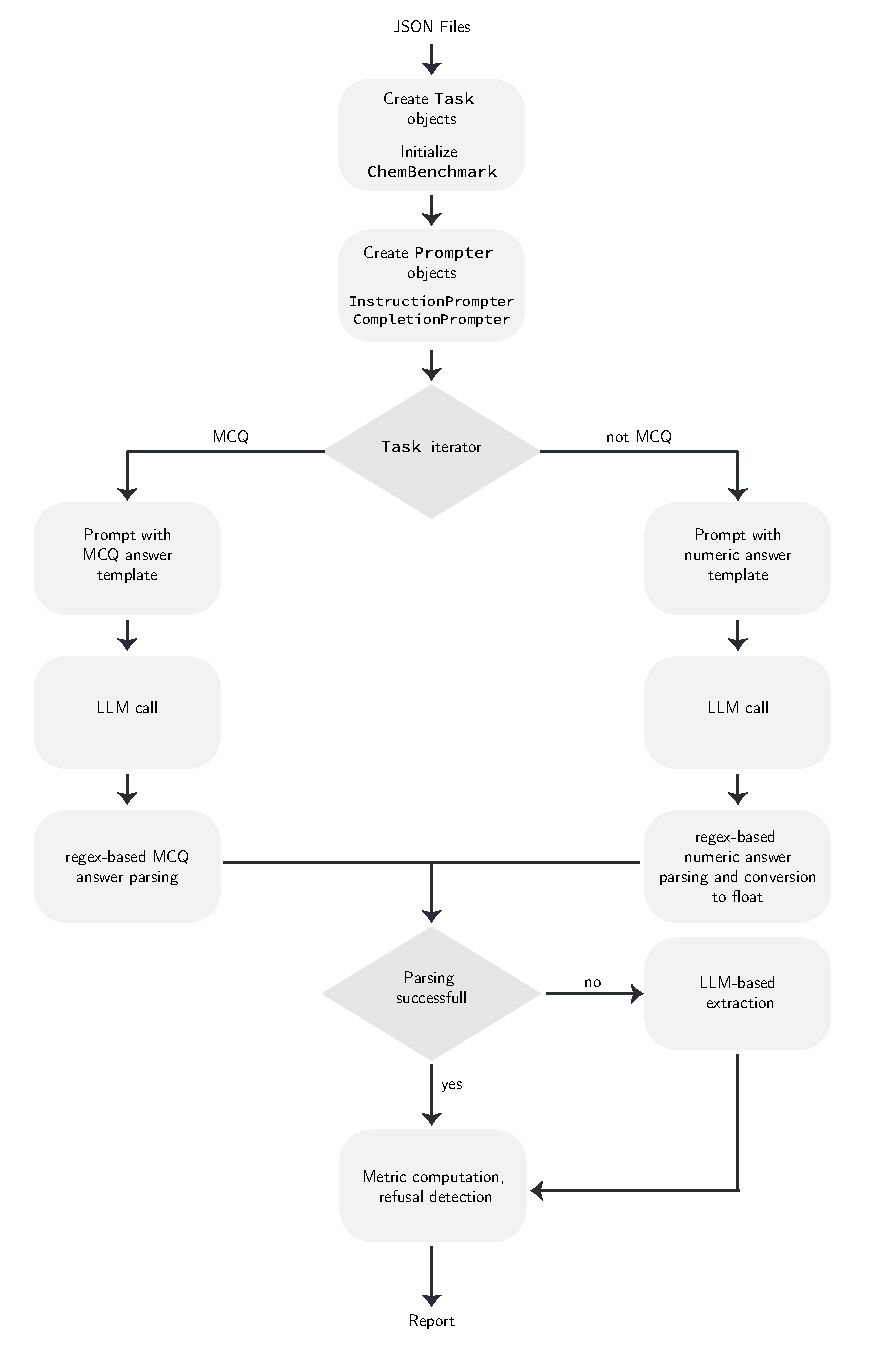
\includegraphics[height=.7\textheight]{figures/process.pdf}
    \caption{\textbf{Overview of the benchmarking pipeline implemented in \chembench.} The process begins with JSON files containing task data, which are used to create \texttt{Task} objects and initialize the \texttt{ChemBenchmark}. \texttt{Prompter} objects are then created to handle different types of prompts for instruction-tuned and completion models.
    The \texttt{Task} Iterator differentiates between \gls{mcq} and other question types. For each task type, appropriate prompts are generated and passed to the \gls{llm}. The responses are then processed using regex-based parsing methods specific to \gls{mcq} or numeric answers (after obtaining the relevant part of the response from the instruction-tuned models).
    The regex-based parsing is elaborate and also able to handle special cases such as scientific notation, or roman numerals.
    If the initial parsing is unsuccessful, the system employs an \gls{llm}-based extraction method as a fallback. The parsed or extracted answers then undergo metric computation and refusal detection.}
    \label{fig:process}
\end{figure}



\clearpage
\subsection{Human baseline} \label{sec:human_baseline}
\paragraph{App} To facilitate the collection of responses, we developed a responsive web application in Typescript using the Next.js\autocite{nextjs} app router framework.
This application handles serving the user interface and exposes various \gls{rest} \glspl{api} for relevant operations.
We utilize a Postgresql.
The web application is styled with Tailwind CSS\autocite{tailwindcss} using the shadcn/ui component library and uses NextAuth\autocite{nextauth} for easy and secure user authentication.
The application is hosted on the Vercel web hosting platform.

In the applications, human participants were presented with molecules as rendered drawings and SMILES strings. \LaTeX\xspace equations and chemical equations were rendered using MathJax (\Cref{fig:screenshots}).


\begin{figure}
    \subfloat[A physcial chemistry question.]{
        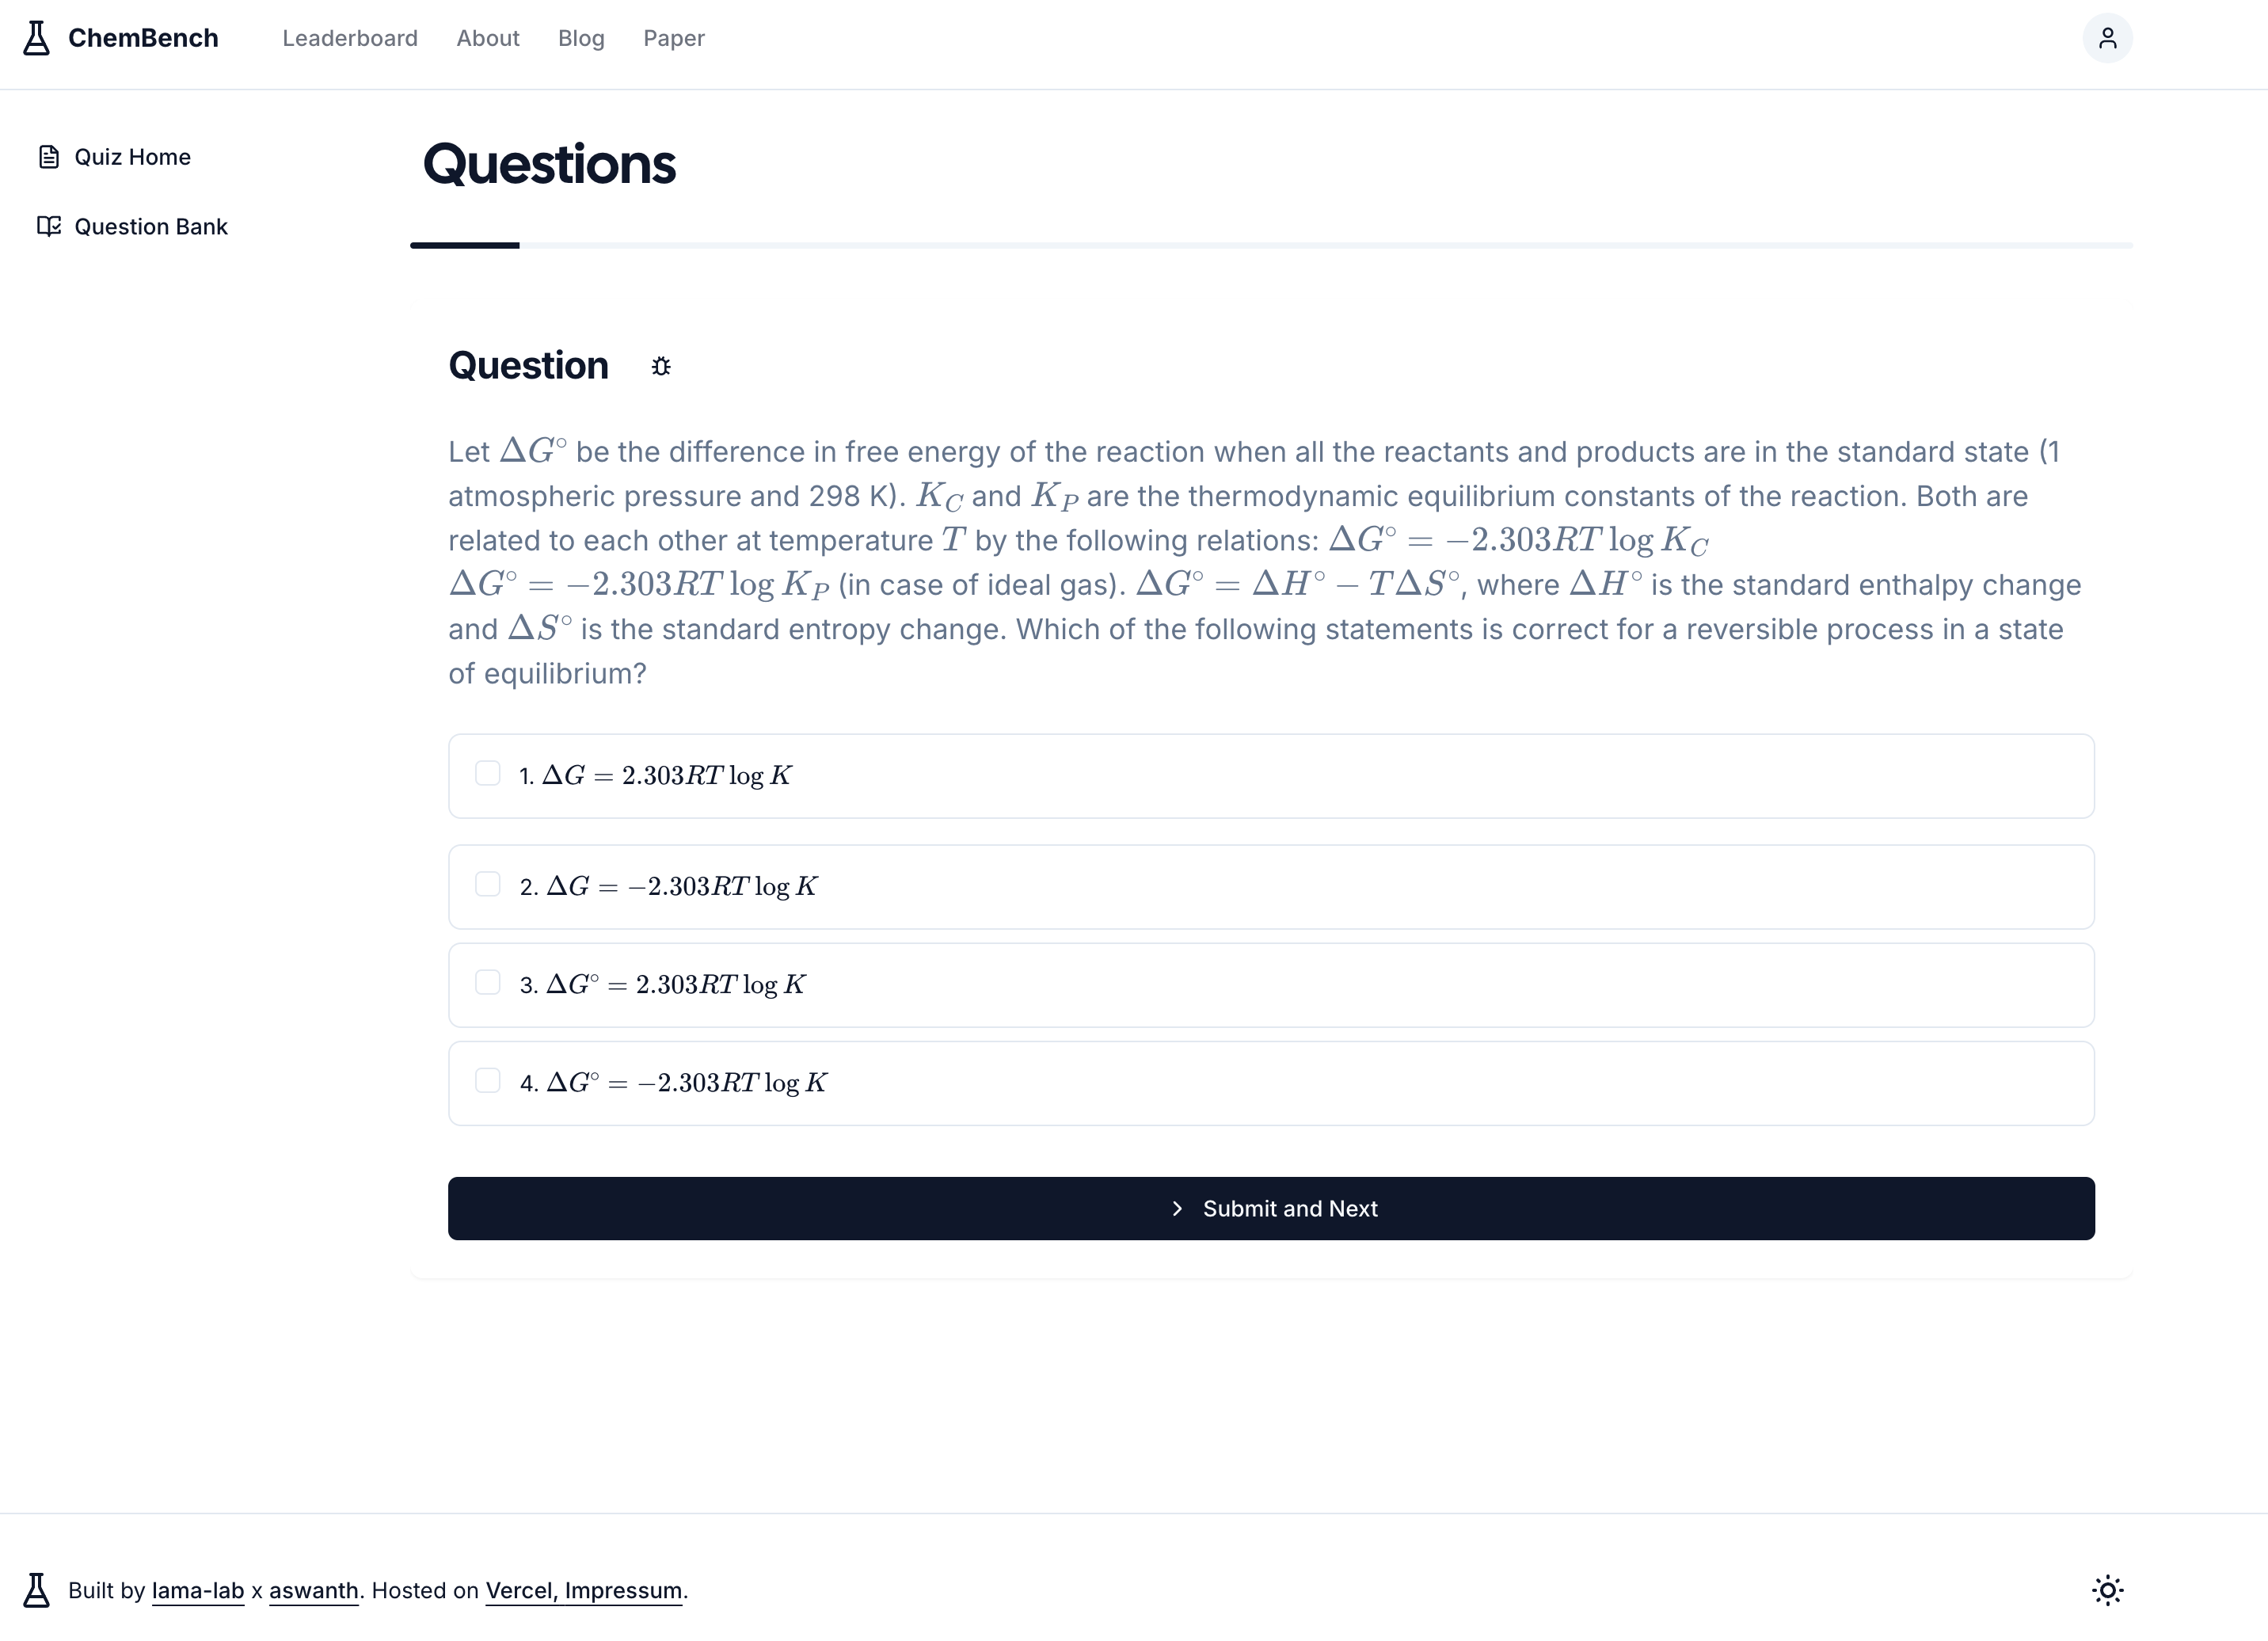
\includegraphics[width=\textwidth]{figures/screenshot_a.png}
    }

    \subfloat[An organic chemistry question.]{
        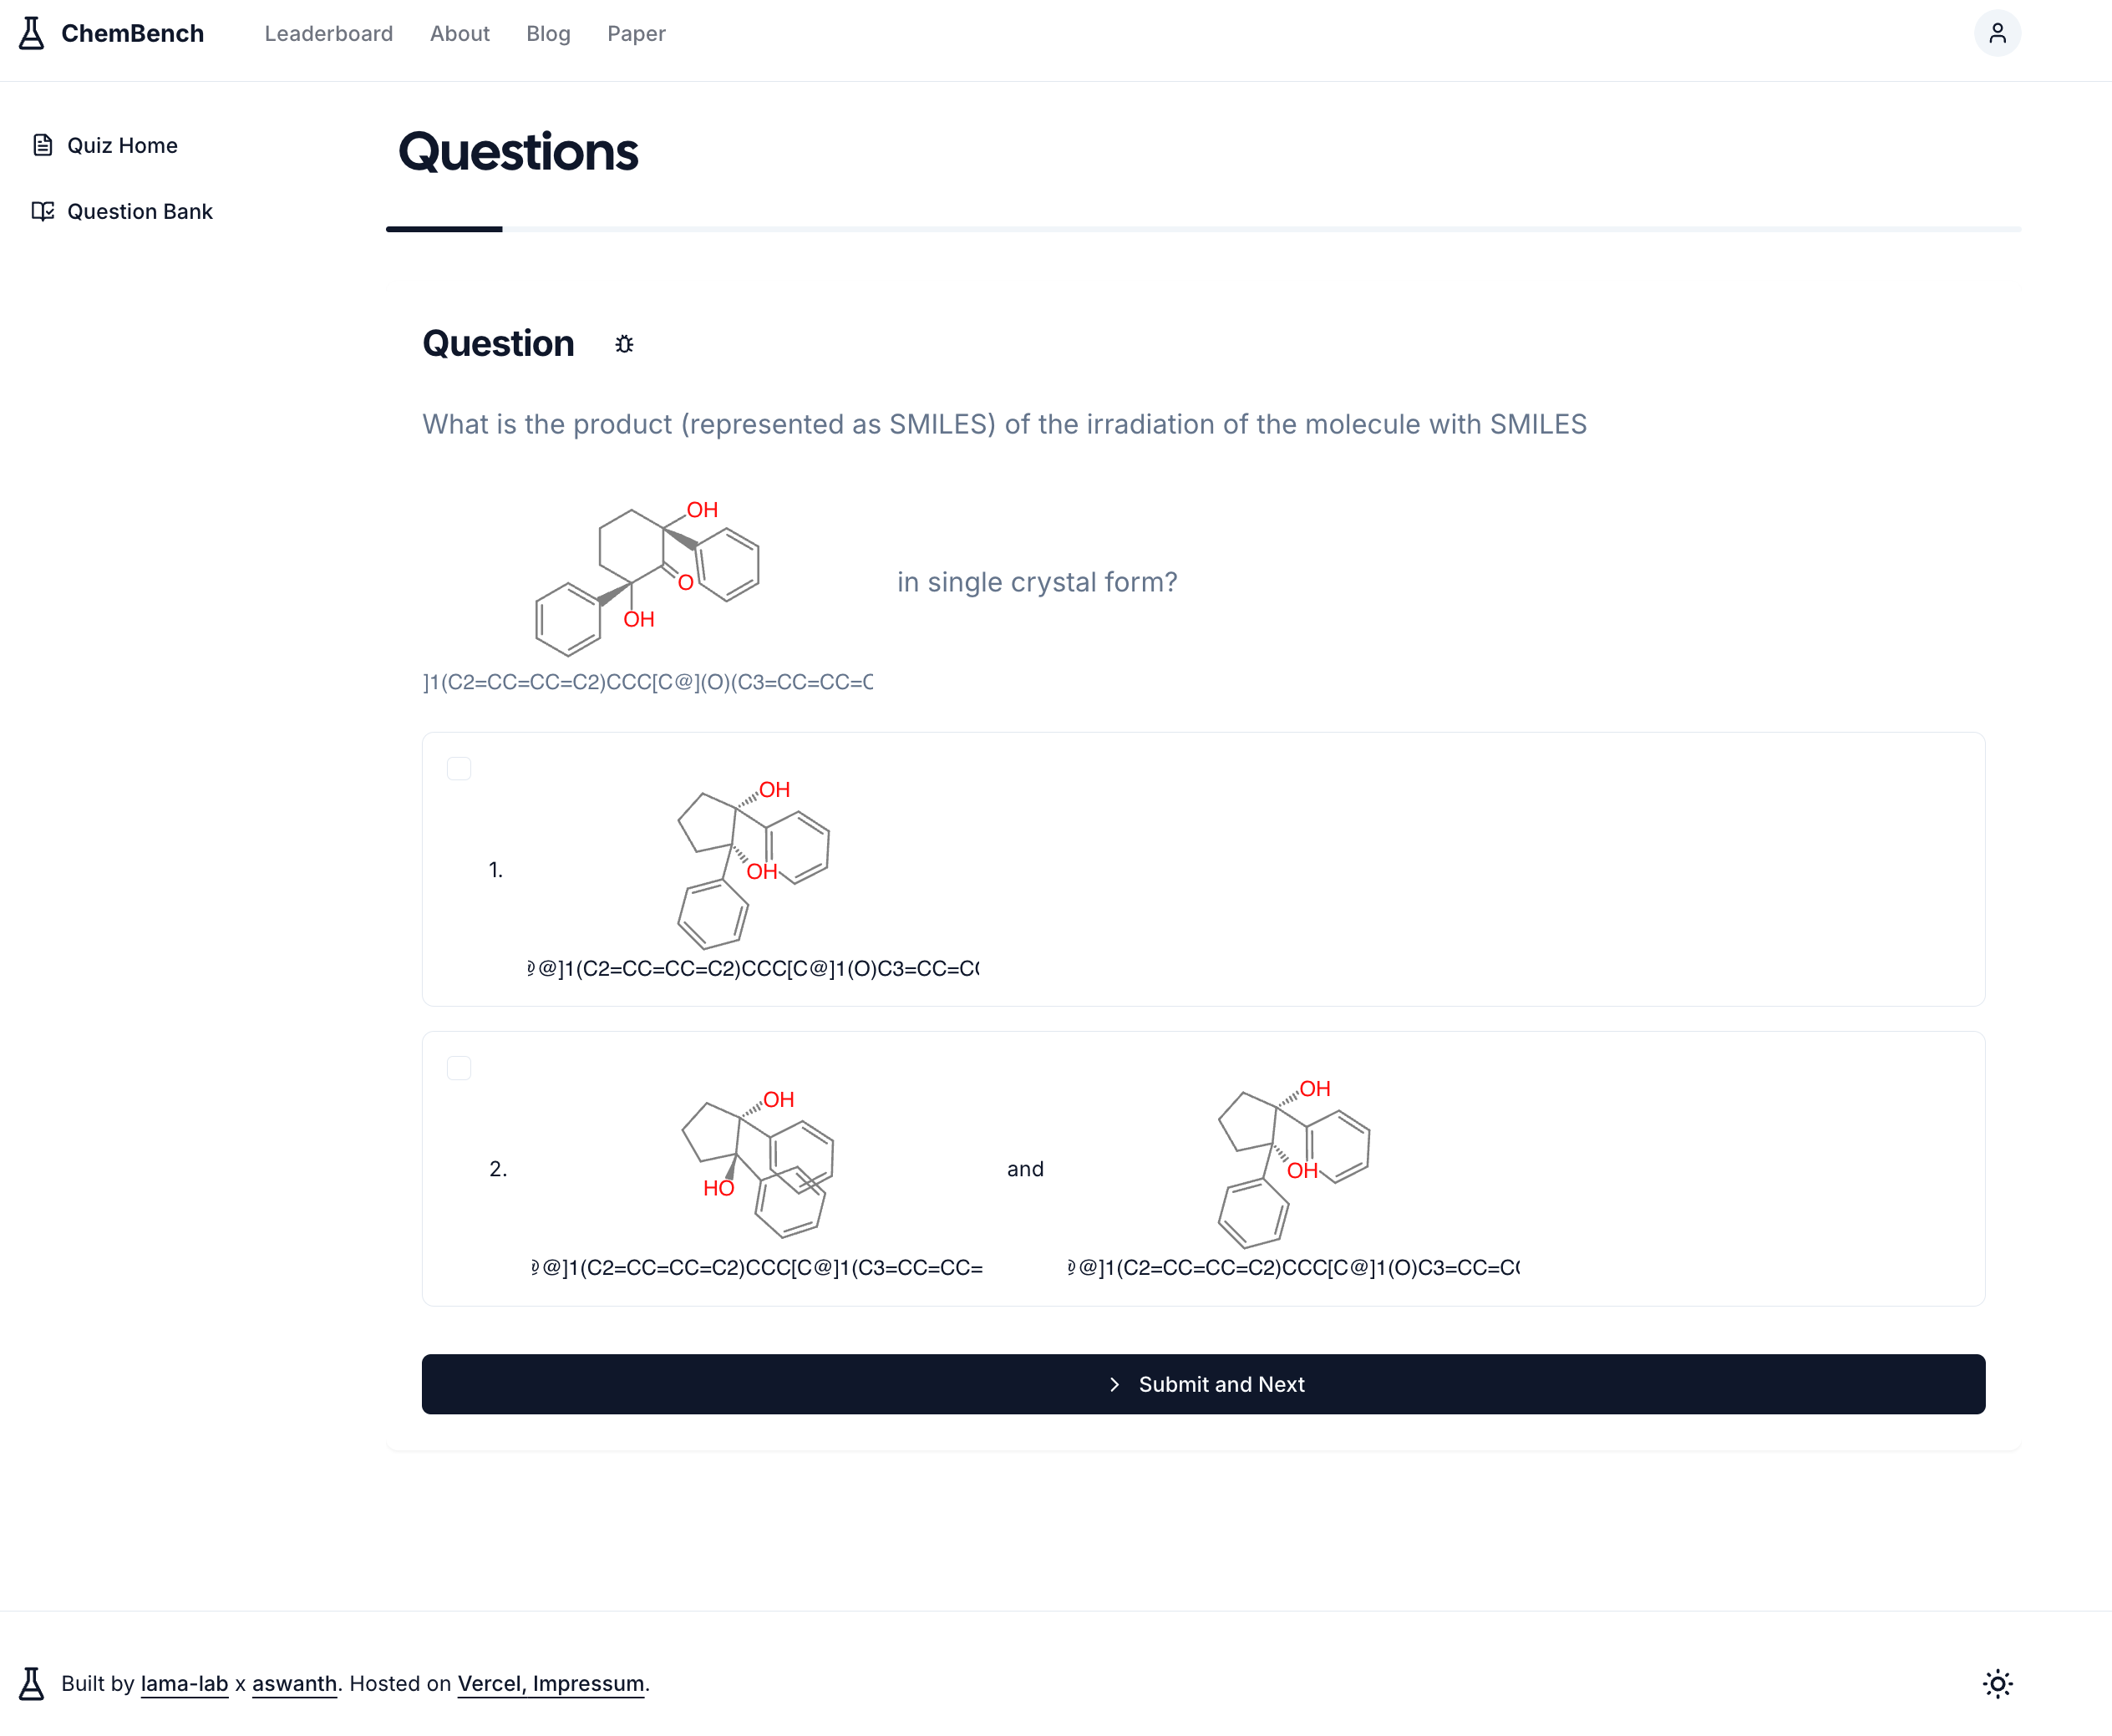
\includegraphics[width=\textwidth]{figures/screenshot_b.png}
    }
    \caption{\textbf{Examples of how questions were shown to the human participants.}}
    \label{fig:screenshots}
\end{figure}

\paragraph{Statistics}
\Cref{fig:human_score_distribution} shows the distribution of scores our human scorers achieved.

\begin{figure}[htb]
    \centering
    \includegraphics{figures/human_score_distribution.pdf}
    \script{plot_human_score_distribution.py}
    \caption{\textbf{Distribution of human scores.} The histogram and kernel density estimates show the fraction of questions answered correctly by the human volunteers.
    Since the best possible score for each question is one and the worst possible score is zero, the values on this plot are between zero and one. A score of one would mean that a volunteer answered all questions correctly. A score of zero would mean that no question was answered correctly.
    We find that the scores for the questions that the human volunteers answered with tools are generally lower than the scores for the questions that the human volunteers answered without tools.
    }
    \label{fig:human_score_distribution}
\end{figure}

We also recorded the time humans took to answer the questions. This time is the time from the question being displayed to the human to the human submitting the answer.

\begin{figure}[htb]
    \centering
    \includegraphics{figures/human_timing.pdf}
    \script{analyze_human_data.py}
    \caption{\textbf{Time taken by human scorers to answer questions vs.\ correctness of their answers.} From the plot, it is clear that there is no clear dependence of the correctness of the answers on the time taken by the human scorers to answer the questions. However, we see that human scorers typically took longer to correctly answer questions with tool use.}
    \label{fig:human_timing}
\end{figure}

Additionally, we prompted users to provide additional information about their experience in chemistry.
While we recorded fine-grained information, e.g., their specialization, we focused on the number of years since the first university-level chemistry course.
\Cref{fig:experience_vs_correctness} shows that the experience of the human scorers was weakly correlated with the correctness of their answers (\Cref{fig:experience_vs_correctness}, Spearman's \(\rho \approx \variable{output/spearman_experience_score.txt}\), and \(p \approx \variable{output/spearman_experience_score_p.txt}\)).

\begin{figure}[htb]
    \centering
    \includegraphics{figures/experience_vs_correctness.pdf}
    \script{analyze_human_data.py}
    \caption{\textbf{Experience of human  scorers vs.\ correctness of their answers.} The experience (in the number of years since the first university-level chemistry course) of the human scorers wasp correlated with the correctness of their answers.}
    \label{fig:experience_vs_correctness}
\end{figure}

\paragraph{Tool use}
In our study, humans were allowed to use tools for answering some questions.
They could also report what tools they used for answering questions. As \Cref{fig:tool_use} shows, the most commonly tool was some form of web search (which, according to the freetext responses, often was a multi-step process).

\begin{figure}
    \centering
    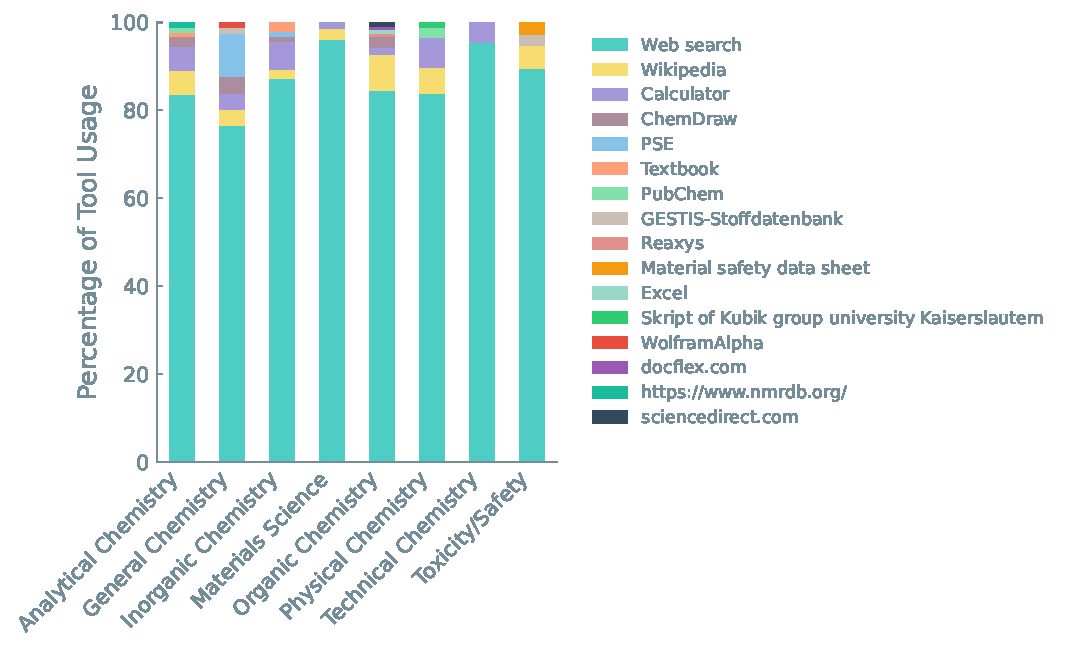
\includegraphics[width=\textwidth]{figures/human_tool_usage_by_topic.pdf}
    \script{human_tool_usage.py}
    \caption{\textbf{Tool usage by human scorers.} The plot shows the most commonly used tools by human participants.}
    \label{fig:tool_use}
\end{figure}

\clearpage
\subsection{Confidence estimates} \label{sec:confidence_estimates}

Since it is important to understand if models can provide an indication of whether their answer might likely be incorrect, we prompted some of our top performing \glspl{llm} to return the confidence in providing a correct answer on an ordinal scale.
This is similar to the verbalized confidence scores reported by \textcite{xiong2023llms}.
We find that the models show different distributions of confidence scores, which, for some, are skewed to the extremes.

In addition, we also analyzed the confidence estimated via the log probabilities of the answer tokens. This probability of a token given the context is not necessarily the same as the confidence in the correctness of the answer. However, it is still often used as a proxy.

Our analysis of both log probabilities and prompting confidence reveals distinct calibration behaviors across different language models.
\GPTFourO demonstrates an overconfident tendency, often assigning high probabilities even to incorrect answers.
However, when \GPTFourO displays high confidence, it accurately predicts correct answers approximately \SI{80}{\percent} of the time. In contrast, \LlamaThreeOneEightBInstruct confidence distribution is more evenly spread, with a majority of predictions centered around 0.5. High-confidence predictions from \LlamaThreeOneEightBInstruct are less frequent compared to \GPTFourO, and unlike \GPTFourO, high confidence does not necessarily correlate with a higher chance of correct answers.

\begin{figure}[htb]
    \centering
    \includegraphics[width=\textwidth]{figures/log_probs_calibration_plot_overall_filtered.pdf}
    \caption{\textbf{Reliability diagram of histogram of logit-based confidence estimates.} For this analysis we obtained the linear probability from the logprobs of the models. Only logprobs of the tokens corresponding to the answers were considered. Linear proabability was computed by taking exponential of logprobs (for sequences with multiple tokens, values were multiplied).  The plot shows the average predicted probability and the fraction of correct answers for each bin of linear probabilities. The ideal scenario is a diagonal line, indicating perfect calibration where the model's confidence aligns perfectly with the actual correctness. The \gls{ece} value quantifies the overall calibration performance, with a lower \gls{ece} indicating better calibration.}
    \label{fig:confidence_score_distributions}
    \script{plot_logprobs.py}
\end{figure}

\clearpage
\subsection{Impact of sampling temperature}
We also investigated the impact of sampling temperature (i.e. temperature 0 means always sampling the most likely token, higher temperatures introduce some randomness in the generation process) on the performance of the models. \Cref{fig:temperature_impact} shows that, generally, the performance of models tends to decrease with increasing temperature.

\begin{figure}[!h]
    \centering
    \includegraphics{figures/swarm_plot_combined.pdf}
    \caption{\textbf{Impact of sampling temperature on the performance of the models.} The plot shows the performance of the models at zero temperature (i.e., greedy decoding) and temperature of one. The performance is measured in terms of the fraction of questions answered correctly.}
    \label{fig:temperature_impact}
    \script{plot_temperature_diffs.py}
\end{figure}





\clearpage
\subsection{Leaderboard}
Our leaderboard is based on the tool chain developed for Matbench.\autocite{Dunn_2020}
Briefly, the \chembench pipeline produces standardized files in \texttt{json} format that contributors can add via pull requests to the \chembench repository.
The Markdown tables and interactive plots are automatically generated and updated on the \chembench website. The leaderboard is available at \url{https://lamalab-org.github.io/chem-bench/leaderboard/}.

\clearpage

\printnoidxglossary[type=\acronymtype, nonumberlist]  % https://github.com/tectonic-typesetting/tectonic/issues/704


\bibliography{references}

\end{document}
